% Options for packages loaded elsewhere
\PassOptionsToPackage{unicode}{hyperref}
\PassOptionsToPackage{hyphens}{url}
%
\documentclass[
]{article}
\usepackage{lmodern}
\usepackage{amssymb,amsmath}
\usepackage{ifxetex,ifluatex}
\ifnum 0\ifxetex 1\fi\ifluatex 1\fi=0 % if pdftex
  \usepackage[T1]{fontenc}
  \usepackage[utf8]{inputenc}
  \usepackage{textcomp} % provide euro and other symbols
\else % if luatex or xetex
  \usepackage{unicode-math}
  \defaultfontfeatures{Scale=MatchLowercase}
  \defaultfontfeatures[\rmfamily]{Ligatures=TeX,Scale=1}
\fi
% Use upquote if available, for straight quotes in verbatim environments
\IfFileExists{upquote.sty}{\usepackage{upquote}}{}
\IfFileExists{microtype.sty}{% use microtype if available
  \usepackage[]{microtype}
  \UseMicrotypeSet[protrusion]{basicmath} % disable protrusion for tt fonts
}{}
\makeatletter
\@ifundefined{KOMAClassName}{% if non-KOMA class
  \IfFileExists{parskip.sty}{%
    \usepackage{parskip}
  }{% else
    \setlength{\parindent}{0pt}
    \setlength{\parskip}{6pt plus 2pt minus 1pt}}
}{% if KOMA class
  \KOMAoptions{parskip=half}}
\makeatother
\usepackage{xcolor}
\IfFileExists{xurl.sty}{\usepackage{xurl}}{} % add URL line breaks if available
\IfFileExists{bookmark.sty}{\usepackage{bookmark}}{\usepackage{hyperref}}
\hypersetup{
  pdftitle={Final},
  pdfauthor={Zachary Palmore},
  hidelinks,
  pdfcreator={LaTeX via pandoc}}
\urlstyle{same} % disable monospaced font for URLs
\usepackage[margin=1in]{geometry}
\usepackage{color}
\usepackage{fancyvrb}
\newcommand{\VerbBar}{|}
\newcommand{\VERB}{\Verb[commandchars=\\\{\}]}
\DefineVerbatimEnvironment{Highlighting}{Verbatim}{commandchars=\\\{\}}
% Add ',fontsize=\small' for more characters per line
\usepackage{framed}
\definecolor{shadecolor}{RGB}{248,248,248}
\newenvironment{Shaded}{\begin{snugshade}}{\end{snugshade}}
\newcommand{\AlertTok}[1]{\textcolor[rgb]{0.94,0.16,0.16}{#1}}
\newcommand{\AnnotationTok}[1]{\textcolor[rgb]{0.56,0.35,0.01}{\textbf{\textit{#1}}}}
\newcommand{\AttributeTok}[1]{\textcolor[rgb]{0.77,0.63,0.00}{#1}}
\newcommand{\BaseNTok}[1]{\textcolor[rgb]{0.00,0.00,0.81}{#1}}
\newcommand{\BuiltInTok}[1]{#1}
\newcommand{\CharTok}[1]{\textcolor[rgb]{0.31,0.60,0.02}{#1}}
\newcommand{\CommentTok}[1]{\textcolor[rgb]{0.56,0.35,0.01}{\textit{#1}}}
\newcommand{\CommentVarTok}[1]{\textcolor[rgb]{0.56,0.35,0.01}{\textbf{\textit{#1}}}}
\newcommand{\ConstantTok}[1]{\textcolor[rgb]{0.00,0.00,0.00}{#1}}
\newcommand{\ControlFlowTok}[1]{\textcolor[rgb]{0.13,0.29,0.53}{\textbf{#1}}}
\newcommand{\DataTypeTok}[1]{\textcolor[rgb]{0.13,0.29,0.53}{#1}}
\newcommand{\DecValTok}[1]{\textcolor[rgb]{0.00,0.00,0.81}{#1}}
\newcommand{\DocumentationTok}[1]{\textcolor[rgb]{0.56,0.35,0.01}{\textbf{\textit{#1}}}}
\newcommand{\ErrorTok}[1]{\textcolor[rgb]{0.64,0.00,0.00}{\textbf{#1}}}
\newcommand{\ExtensionTok}[1]{#1}
\newcommand{\FloatTok}[1]{\textcolor[rgb]{0.00,0.00,0.81}{#1}}
\newcommand{\FunctionTok}[1]{\textcolor[rgb]{0.00,0.00,0.00}{#1}}
\newcommand{\ImportTok}[1]{#1}
\newcommand{\InformationTok}[1]{\textcolor[rgb]{0.56,0.35,0.01}{\textbf{\textit{#1}}}}
\newcommand{\KeywordTok}[1]{\textcolor[rgb]{0.13,0.29,0.53}{\textbf{#1}}}
\newcommand{\NormalTok}[1]{#1}
\newcommand{\OperatorTok}[1]{\textcolor[rgb]{0.81,0.36,0.00}{\textbf{#1}}}
\newcommand{\OtherTok}[1]{\textcolor[rgb]{0.56,0.35,0.01}{#1}}
\newcommand{\PreprocessorTok}[1]{\textcolor[rgb]{0.56,0.35,0.01}{\textit{#1}}}
\newcommand{\RegionMarkerTok}[1]{#1}
\newcommand{\SpecialCharTok}[1]{\textcolor[rgb]{0.00,0.00,0.00}{#1}}
\newcommand{\SpecialStringTok}[1]{\textcolor[rgb]{0.31,0.60,0.02}{#1}}
\newcommand{\StringTok}[1]{\textcolor[rgb]{0.31,0.60,0.02}{#1}}
\newcommand{\VariableTok}[1]{\textcolor[rgb]{0.00,0.00,0.00}{#1}}
\newcommand{\VerbatimStringTok}[1]{\textcolor[rgb]{0.31,0.60,0.02}{#1}}
\newcommand{\WarningTok}[1]{\textcolor[rgb]{0.56,0.35,0.01}{\textbf{\textit{#1}}}}
\usepackage{graphicx,grffile}
\makeatletter
\def\maxwidth{\ifdim\Gin@nat@width>\linewidth\linewidth\else\Gin@nat@width\fi}
\def\maxheight{\ifdim\Gin@nat@height>\textheight\textheight\else\Gin@nat@height\fi}
\makeatother
% Scale images if necessary, so that they will not overflow the page
% margins by default, and it is still possible to overwrite the defaults
% using explicit options in \includegraphics[width, height, ...]{}
\setkeys{Gin}{width=\maxwidth,height=\maxheight,keepaspectratio}
% Set default figure placement to htbp
\makeatletter
\def\fps@figure{htbp}
\makeatother
\setlength{\emergencystretch}{3em} % prevent overfull lines
\providecommand{\tightlist}{%
  \setlength{\itemsep}{0pt}\setlength{\parskip}{0pt}}
\setcounter{secnumdepth}{-\maxdimen} % remove section numbering
\usepackage{booktabs}
\usepackage{longtable}
\usepackage{array}
\usepackage{multirow}
\usepackage{wrapfig}
\usepackage{float}
\usepackage{colortbl}
\usepackage{pdflscape}
\usepackage{tabu}
\usepackage{threeparttable}
\usepackage{threeparttablex}
\usepackage[normalem]{ulem}
\usepackage{makecell}
\usepackage{xcolor}

\title{Final}
\author{Zachary Palmore}
\date{5/20/2021}

\begin{document}
\maketitle

\begin{Shaded}
\begin{Highlighting}[]
\KeywordTok{library}\NormalTok{(tidyverse)}
\KeywordTok{library}\NormalTok{(kableExtra)}
\end{Highlighting}
\end{Shaded}

\hypertarget{problem-1}{%
\subsection{Problem 1}\label{problem-1}}

Using R, generate a random variable X that has 10,000 random uniform
numbers from 1 to N, where N can be any number of your choosing greater
than or equal to 6. Then generate a random variable Y that has 10,000
random normal numbers with a mean of \(\mu=\sigma=(N+1)/2.\)

\begin{Shaded}
\begin{Highlighting}[]
\KeywordTok{set.seed}\NormalTok{(}\DecValTok{41}\NormalTok{)}
\NormalTok{N <-}\StringTok{ }\DecValTok{41} \CommentTok{# Random number greater than or equal to 6}
\NormalTok{n <-}\StringTok{ }\DecValTok{10000} \CommentTok{# Quantity of random normal numbers to generate}
\NormalTok{sigma <-}\StringTok{ }\NormalTok{(N }\OperatorTok{+}\StringTok{ }\DecValTok{1}\NormalTok{)}\OperatorTok{/}\DecValTok{2} \CommentTok{# Sigma}
\NormalTok{mu <-}\StringTok{ }\NormalTok{sigma }\CommentTok{# Mu = Sigma}
\CommentTok{# Generate random number}
\NormalTok{df <-}\StringTok{ }\KeywordTok{data.frame}\NormalTok{(}\DataTypeTok{X =} \KeywordTok{runif}\NormalTok{(n, }\DataTypeTok{min =} \DecValTok{1}\NormalTok{, }\DataTypeTok{max =}\NormalTok{ N), }
                 \DataTypeTok{Y =} \KeywordTok{rnorm}\NormalTok{(n, }\DataTypeTok{mean =}\NormalTok{ mu, }\DataTypeTok{sd =}\NormalTok{ sigma))}
\CommentTok{# Display random numbers}
\KeywordTok{head}\NormalTok{(df, }\DecValTok{10}\NormalTok{)}
\end{Highlighting}
\end{Shaded}

\begin{verbatim}
##            X         Y
## 1   9.539620 21.708869
## 2  39.849134 17.692613
## 3  24.127480 24.785695
## 4   6.683199 21.316268
## 5  34.670271 -8.210459
## 6  39.481321 14.583845
## 7  37.050824 -1.709704
## 8  21.876923 36.841523
## 9  33.698672 30.865059
## 10 27.731654 41.466029
\end{verbatim}

\begin{Shaded}
\begin{Highlighting}[]
\KeywordTok{hist}\NormalTok{(df}\OperatorTok{$}\NormalTok{Y)}
\end{Highlighting}
\end{Shaded}

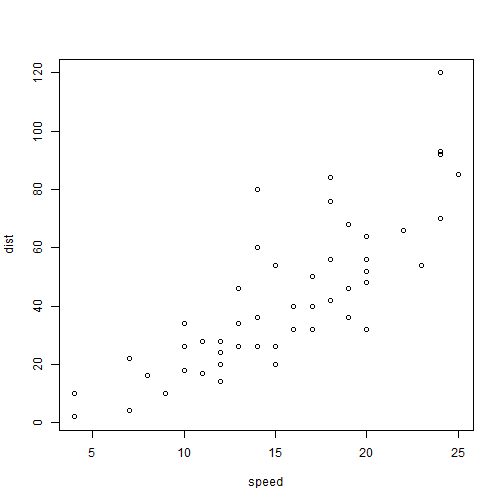
\includegraphics{Final_files/figure-latex/unnamed-chunk-2-1.pdf}

Probability. Calculate as a minimum the below probabilities a through
c.~Assume the small letter ``x'' is estimated as the median of the X
variable, and the small letter ``y'' is estimated as the 1st quartile of
the Y variable. Interpret the meaning of all probabilities.

\[A. \ P(X>x | X>y) \hspace{8pt} B. \ P(X>x, Y>y) \hspace{8pt} C. P(X<x | X>y)\]

If we assume the small letter \(x\) is estimated as the median of X
variable, and the small letter \(y\) is estimated as the 1st quartile of
the Y variable then we have the following values of \(x\) and \(y\) and
can calculate the minimum as such:

\begin{Shaded}
\begin{Highlighting}[]
\NormalTok{x =}\StringTok{ }\KeywordTok{median}\NormalTok{(df}\OperatorTok{$}\NormalTok{X) }\CommentTok{# median of X}
\NormalTok{y =}\StringTok{ }\KeywordTok{quantile}\NormalTok{(df}\OperatorTok{$}\NormalTok{Y, }\FloatTok{0.25}\NormalTok{) }\CommentTok{# 1st quartile of Y}
\CommentTok{# A. P(X>x | X>y)}
\NormalTok{PXxXy <-}\StringTok{ }\NormalTok{df }\OperatorTok\StringTok{ }
\StringTok{  }\KeywordTok{filter}\NormalTok{(X}\OperatorTok{>}\NormalTok{x, X}\OperatorTok{>}\NormalTok{y) }\OperatorTok\StringTok{ }
\StringTok{  }\KeywordTok{nrow}\NormalTok{() }\OperatorTok{/}\StringTok{ }\NormalTok{n}
\NormalTok{PXy <-}\StringTok{ }\NormalTok{df }\OperatorTok\StringTok{ }
\StringTok{  }\KeywordTok{filter}\NormalTok{(X}\OperatorTok{>}\NormalTok{y) }\OperatorTok\StringTok{ }
\StringTok{  }\KeywordTok{nrow}\NormalTok{() }\OperatorTok{/}\StringTok{ }\NormalTok{n }
\NormalTok{A <-}\StringTok{ }\KeywordTok{signif}\NormalTok{((PXxXy }\OperatorTok{/}\StringTok{ }\NormalTok{PXy), }\DecValTok{3}\NormalTok{)}
\CommentTok{# B. P(X>x, Y>y)}
\NormalTok{PXxXy <-}\StringTok{ }\NormalTok{df }\OperatorTok\StringTok{ }
\StringTok{  }\KeywordTok{filter}\NormalTok{(X}\OperatorTok{>}\NormalTok{x, Y}\OperatorTok{>}\NormalTok{y) }\OperatorTok\StringTok{ }
\StringTok{  }\KeywordTok{nrow}\NormalTok{() }\OperatorTok{/}\StringTok{ }\NormalTok{n}
\NormalTok{B <-}\StringTok{ }\KeywordTok{signif}\NormalTok{(PXxXy, }\DecValTok{3}\NormalTok{)}
\CommentTok{# C. P(X<x | X>y)}
\NormalTok{PXxXy <-}\StringTok{ }\NormalTok{df }\OperatorTok\StringTok{ }
\StringTok{  }\KeywordTok{filter}\NormalTok{(X }\OperatorTok{<}\StringTok{ }\NormalTok{x, }
\NormalTok{         X }\OperatorTok{>}\StringTok{ }\NormalTok{y) }\OperatorTok\StringTok{ }
\StringTok{  }\KeywordTok{nrow}\NormalTok{() }\OperatorTok{/}\StringTok{ }\NormalTok{n}
\NormalTok{PXy <-}\StringTok{ }\NormalTok{df }\OperatorTok\StringTok{ }
\StringTok{  }\KeywordTok{filter}\NormalTok{(X }\OperatorTok{>}\StringTok{ }\NormalTok{y) }\OperatorTok\StringTok{ }
\StringTok{  }\KeywordTok{nrow}\NormalTok{() }\OperatorTok{/}\StringTok{ }\NormalTok{n }
\NormalTok{C <-}\StringTok{ }\NormalTok{PXxXy}\OperatorTok{/}\NormalTok{PXy}
\KeywordTok{print}\NormalTok{(}\KeywordTok{paste}\NormalTok{(}\StringTok{"A.:"}\NormalTok{,A,}\StringTok{"B.:"}\NormalTok{,B,}\StringTok{"C.:"}\NormalTok{,C))}
\end{Highlighting}
\end{Shaded}

\begin{verbatim}
## [1] "A.: 0.583 B.: 0.375 C.: 0.417045587035094"
\end{verbatim}

We can interpret the meaning of \(P(X>x | X>y)\) as approximately 0.583.
That is to say (in words), the probability of X\textgreater x given
X\textgreater y is 0.583. For B, where \(P(X>x, Y>y)\) we have 0.375 and
would state verbally that the probability X is greater than x and Y is
greater than y is 0.375. Lastly, for C, where P(X\textgreater x
\textbar{} X\textgreater y), we have 0.4170456 and simply say that the
probability of Xy is 0.4170456.

Investigate whether \(P(X>x and Y>y)=P(X>x)P(Y>y)\) by building a table
and evaluating the marginal and joint probabilities.

\begin{Shaded}
\begin{Highlighting}[]
\CommentTok{# Joint P}
\NormalTok{JAB <-}\StringTok{ }\NormalTok{df }\OperatorTok\StringTok{ }
\StringTok{  }\KeywordTok{mutate}\NormalTok{(}\DataTypeTok{A =} \KeywordTok{ifelse}\NormalTok{(X }\OperatorTok{>}\StringTok{ }\NormalTok{x, }\StringTok{"X > x"}\NormalTok{, }\StringTok{"X < x"}\NormalTok{)) }\OperatorTok\StringTok{ }
\StringTok{  }\KeywordTok{mutate}\NormalTok{(}\DataTypeTok{B =} \KeywordTok{ifelse}\NormalTok{(Y }\OperatorTok{>}\StringTok{ }\NormalTok{y, }\StringTok{" Y > y"}\NormalTok{, }\StringTok{" Y < y"}\NormalTok{)) }\OperatorTok\StringTok{ }
\StringTok{  }\KeywordTok{group_by}\NormalTok{(A, B) }\OperatorTok\StringTok{ }
\StringTok{  }\KeywordTok{summarise}\NormalTok{(}\DataTypeTok{total =} \KeywordTok{n}\NormalTok{()) }\OperatorTok\StringTok{ }
\StringTok{  }\KeywordTok{mutate}\NormalTok{(}\DataTypeTok{P =}\NormalTok{ total }\OperatorTok{/}\StringTok{ }\NormalTok{n)}
\CommentTok{# Marginal P}
\NormalTok{MA <-}\StringTok{ }\NormalTok{JAB }\OperatorTok\StringTok{ }
\StringTok{  }\KeywordTok{ungroup}\NormalTok{() }\OperatorTok\StringTok{ }
\StringTok{  }\KeywordTok{group_by}\NormalTok{(A) }\OperatorTok\StringTok{ }
\StringTok{  }\KeywordTok{summarise}\NormalTok{(}\DataTypeTok{sum =} \KeywordTok{sum}\NormalTok{(total), }\DataTypeTok{P =} \KeywordTok{sum}\NormalTok{(P))}
\NormalTok{MB <-}\StringTok{ }\NormalTok{JAB }\OperatorTok\StringTok{ }
\StringTok{  }\KeywordTok{ungroup}\NormalTok{() }\OperatorTok\StringTok{ }
\StringTok{  }\KeywordTok{group_by}\NormalTok{(B) }\OperatorTok\StringTok{ }
\StringTok{  }\KeywordTok{summarise}\NormalTok{(}\DataTypeTok{sum =} \KeywordTok{sum}\NormalTok{(total), }\DataTypeTok{P =} \KeywordTok{sum}\NormalTok{(P))}
\CommentTok{# build a table}
\NormalTok{tbl <-}\StringTok{ }\KeywordTok{bind_rows}\NormalTok{(JAB, MA, MB) }\OperatorTok\StringTok{ }
\StringTok{  }\KeywordTok{select}\NormalTok{(}\OperatorTok{-}\NormalTok{total) }\OperatorTok\StringTok{ }
\StringTok{  }\KeywordTok{spread}\NormalTok{(A, P) }
\KeywordTok{colnames}\NormalTok{(tbl) <-}\StringTok{ }\KeywordTok{c}\NormalTok{(}\StringTok{"Condition"}\NormalTok{, }\StringTok{"sum"}\NormalTok{, }\StringTok{"X<x"}\NormalTok{, }\StringTok{"X>x"}\NormalTok{, }\StringTok{"Total"}\NormalTok{)}
\KeywordTok{kable}\NormalTok{(tbl)}
\end{Highlighting}
\end{Shaded}

\begin{tabular}{l|r|r|r|r}
\hline
Condition & sum & X<x & X>x & Total\\
\hline
Y < y & 2500 & NA & NA & 0.25\\
\hline
Y < y & NA & 0.125 & 0.125 & NA\\
\hline
Y > y & 7500 & NA & NA & 0.75\\
\hline
Y > y & NA & 0.375 & 0.375 & NA\\
\hline
NA & 5000 & 0.500 & 0.500 & NA\\
\hline
\end{tabular}

They are the approximately the same. Close enough that we can state
\(P(X>x and Y>y)=P(X>x)P(Y>y)\).

Check to see if independence holds by using Fisher's Exact Test and the
Chi Square Test. What is the difference between the two? Which is most
appropriate?

\begin{Shaded}
\begin{Highlighting}[]
\NormalTok{xy <-}\StringTok{ }\KeywordTok{table}\NormalTok{(df}\OperatorTok{$}\NormalTok{X}\OperatorTok{>}\NormalTok{x, df}\OperatorTok{$}\NormalTok{Y}\OperatorTok{>}\NormalTok{y)}
\KeywordTok{chisq.test}\NormalTok{(xy, }\DataTypeTok{correct=}\NormalTok{T)}
\end{Highlighting}
\end{Shaded}

\begin{verbatim}
## 
##  Pearson's Chi-squared test
## 
## data:  xy
## X-squared = 0, df = 1, p-value = 1
\end{verbatim}

\begin{Shaded}
\begin{Highlighting}[]
\KeywordTok{fisher.test}\NormalTok{(xy,}\DataTypeTok{simulate.p.value=}\NormalTok{T)}
\end{Highlighting}
\end{Shaded}

\begin{verbatim}
## 
##  Fisher's Exact Test for Count Data
## 
## data:  xy
## p-value = 1
## alternative hypothesis: true odds ratio is not equal to 1
## 95 percent confidence interval:
##  0.9124854 1.0959080
## sample estimates:
## odds ratio 
##          1
\end{verbatim}

Chi-squared is most appropriate due to sample size and independence
holds with large p-value.

\hypertarget{problem-2}{%
\subsection{Problem 2}\label{problem-2}}

You are to register for Kaggle.com (free) and compete in the House
Prices: Advanced Regression Techniques competition.
\url{https://www.kaggle.com/c/house-prices-advanced-regression-techniques}
. I want you to do the following.

\$\^{}\{1\}\$5 points. Descriptive and Inferential Statistics. Provide
univariate descriptive statistics and appropriate plots for the training
data set. Provide a scatterplot matrix for at least two of the
independent variables and the dependent variable. Derive a correlation
matrix for any three quantitative variables in the dataset. Test the
hypotheses that the correlations between each pairwise set of variables
is 0 and provide an 80\% confidence interval. Discuss the meaning of
your analysis. Would you be worried about familywise error? Why or why
not?

\$\^{}\{2\}\$5 points. Linear Algebra and Correlation. Invert your
correlation matrix from above. (This is known as the precision matrix
and contains variance inflation factors on the diagonal.) Multiply the
correlation matrix by the precision matrix, and then multiply the
precision matrix by the correlation matrix. Conduct LU decomposition on
the matrix.

\$\^{}\{3\}\$5 points. Calculus-Based Probability \& Statistics. Many
times, it makes sense to fit a closed form distribution to data. Select
a variable in the Kaggle.com training dataset that is skewed to the
right, shift it so that the minimum value is absolutely above zero if
necessary. Then load the MASS package and run fitdistr to fit an
exponential probability density function. (See
\url{https://stat.ethz.ch/R-manual/R-devel/library/MASS/html/fitdistr.html}
). Find the optimal value of  for this distribution, and then take 1000
samples from this exponential distribution using this value (e.g.,
rexp(1000, )). Plot a histogram and compare it with a histogram of your
original variable. Using the exponential pdf, find the 5th and 95th
percentiles using the cumulative distribution function (CDF). Also
generate a 95\% confidence interval from the empirical data, assuming
normality. Finally, provide the empirical 5th percentile and 95th
percentile of the data. Discuss.

\$\^{}\{4\}\$10 points. Modeling. Build some type of multiple regression
model and submit your model to the competition board. Provide your
complete model summary and results with analysis. Report your Kaggle.com
user name and score.

\begin{Shaded}
\begin{Highlighting}[]
\CommentTok{# Packages}
\KeywordTok{library}\NormalTok{(psych)}
\KeywordTok{library}\NormalTok{(corrplot)}
\KeywordTok{library}\NormalTok{(matrixcalc)}
\KeywordTok{library}\NormalTok{(MASS)}
\KeywordTok{theme_set}\NormalTok{(}\KeywordTok{theme_minimal}\NormalTok{())}
\end{Highlighting}
\end{Shaded}

\hypertarget{section-1-descriptive-and-inferential-statistics}{%
\subsubsection{Section 1: Descriptive and Inferential
Statistics}\label{section-1-descriptive-and-inferential-statistics}}

\begin{Shaded}
\begin{Highlighting}[]
\CommentTok{# Load the data}
\NormalTok{train <-}\StringTok{ }\KeywordTok{read.csv}\NormalTok{(}\StringTok{"https://raw.githubusercontent.com/palmorezm/msds/main/605/train.csv"}\NormalTok{)}
\NormalTok{test <-}\StringTok{ }\KeywordTok{read.csv}\NormalTok{(}\StringTok{"https://raw.githubusercontent.com/palmorezm/msds/main/605/test.csv"}\NormalTok{)}
\end{Highlighting}
\end{Shaded}

\begin{Shaded}
\begin{Highlighting}[]
\CommentTok{# univariate descriptive statistics for training set}
\KeywordTok{describe}\NormalTok{(train)}
\end{Highlighting}
\end{Shaded}

\begin{verbatim}
##                vars    n      mean       sd   median   trimmed      mad   min
## Id                1 1460    730.50   421.61    730.5    730.50   541.15     1
## MSSubClass        2 1460     56.90    42.30     50.0     49.15    44.48    20
## MSZoning*         3 1460      4.03     0.63      4.0      4.06     0.00     1
## LotFrontage       4 1201     70.05    24.28     69.0     68.94    16.31    21
## LotArea           5 1460  10516.83  9981.26   9478.5   9563.28  2962.23  1300
## Street*           6 1460      2.00     0.06      2.0      2.00     0.00     1
## Alley*            7   91      1.45     0.50      1.0      1.44     0.00     1
## LotShape*         8 1460      2.94     1.41      4.0      3.05     0.00     1
## LandContour*      9 1460      3.78     0.71      4.0      4.00     0.00     1
## Utilities*       10 1460      1.00     0.03      1.0      1.00     0.00     1
## LotConfig*       11 1460      4.02     1.62      5.0      4.27     0.00     1
## LandSlope*       12 1460      1.06     0.28      1.0      1.00     0.00     1
## Neighborhood*    13 1460     13.15     5.89     13.0     13.11     7.41     1
## Condition1*      14 1460      3.03     0.87      3.0      3.00     0.00     1
## Condition2*      15 1460      3.01     0.26      3.0      3.00     0.00     1
## BldgType*        16 1460      1.49     1.20      1.0      1.14     0.00     1
## HouseStyle*      17 1460      4.04     1.91      3.0      4.03     1.48     1
## OverallQual      18 1460      6.10     1.38      6.0      6.08     1.48     1
## OverallCond      19 1460      5.58     1.11      5.0      5.48     0.00     1
## YearBuilt        20 1460   1971.27    30.20   1973.0   1974.13    37.06  1872
## YearRemodAdd     21 1460   1984.87    20.65   1994.0   1986.37    19.27  1950
## RoofStyle*       22 1460      2.41     0.83      2.0      2.26     0.00     1
## RoofMatl*        23 1460      2.08     0.60      2.0      2.00     0.00     1
## Exterior1st*     24 1460     10.62     3.20     13.0     10.93     1.48     1
## Exterior2nd*     25 1460     11.34     3.54     14.0     11.65     2.97     1
## MasVnrType*      26 1452      2.76     0.62      3.0      2.73     0.00     1
## MasVnrArea       27 1452    103.69   181.07      0.0     63.15     0.00     0
## ExterQual*       28 1460      3.54     0.69      4.0      3.65     0.00     1
## ExterCond*       29 1460      4.73     0.73      5.0      4.95     0.00     1
## Foundation*      30 1460      2.40     0.72      2.0      2.46     1.48     1
## BsmtQual*        31 1423      3.26     0.87      3.0      3.43     1.48     1
## BsmtCond*        32 1423      3.81     0.66      4.0      4.00     0.00     1
## BsmtExposure*    33 1422      3.27     1.15      4.0      3.46     0.00     1
## BsmtFinType1*    34 1423      3.73     1.83      3.0      3.79     2.97     1
## BsmtFinSF1       35 1460    443.64   456.10    383.5    386.08   568.58     0
## BsmtFinType2*    36 1422      5.71     0.94      6.0      5.98     0.00     1
## BsmtFinSF2       37 1460     46.55   161.32      0.0      1.38     0.00     0
## BsmtUnfSF        38 1460    567.24   441.87    477.5    519.29   426.99     0
## TotalBsmtSF      39 1460   1057.43   438.71    991.5   1036.70   347.67     0
## Heating*         40 1460      2.04     0.30      2.0      2.00     0.00     1
## HeatingQC*       41 1460      2.54     1.74      1.0      2.42     0.00     1
## CentralAir*      42 1460      1.93     0.25      2.0      2.00     0.00     1
## Electrical*      43 1459      4.68     1.05      5.0      5.00     0.00     1
## X1stFlrSF        44 1460   1162.63   386.59   1087.0   1129.99   347.67   334
## X2ndFlrSF        45 1460    346.99   436.53      0.0    285.36     0.00     0
## LowQualFinSF     46 1460      5.84    48.62      0.0      0.00     0.00     0
## GrLivArea        47 1460   1515.46   525.48   1464.0   1467.67   483.33   334
## BsmtFullBath     48 1460      0.43     0.52      0.0      0.39     0.00     0
## BsmtHalfBath     49 1460      0.06     0.24      0.0      0.00     0.00     0
## FullBath         50 1460      1.57     0.55      2.0      1.56     0.00     0
## HalfBath         51 1460      0.38     0.50      0.0      0.34     0.00     0
## BedroomAbvGr     52 1460      2.87     0.82      3.0      2.85     0.00     0
## KitchenAbvGr     53 1460      1.05     0.22      1.0      1.00     0.00     0
## KitchenQual*     54 1460      3.34     0.83      4.0      3.50     0.00     1
## TotRmsAbvGrd     55 1460      6.52     1.63      6.0      6.41     1.48     2
## Functional*      56 1460      6.75     0.98      7.0      7.00     0.00     1
## Fireplaces       57 1460      0.61     0.64      1.0      0.53     1.48     0
## FireplaceQu*     58  770      3.73     1.13      3.0      3.80     1.48     1
## GarageType*      59 1379      3.28     1.79      2.0      3.11     0.00     1
## GarageYrBlt      60 1379   1978.51    24.69   1980.0   1981.07    31.13  1900
## GarageFinish*    61 1379      2.18     0.81      2.0      2.23     1.48     1
## GarageCars       62 1460      1.77     0.75      2.0      1.77     0.00     0
## GarageArea       63 1460    472.98   213.80    480.0    469.81   177.91     0
## GarageQual*      64 1379      4.86     0.61      5.0      5.00     0.00     1
## GarageCond*      65 1379      4.90     0.52      5.0      5.00     0.00     1
## PavedDrive*      66 1460      2.86     0.50      3.0      3.00     0.00     1
## WoodDeckSF       67 1460     94.24   125.34      0.0     71.76     0.00     0
## OpenPorchSF      68 1460     46.66    66.26     25.0     33.23    37.06     0
## EnclosedPorch    69 1460     21.95    61.12      0.0      3.87     0.00     0
## X3SsnPorch       70 1460      3.41    29.32      0.0      0.00     0.00     0
## ScreenPorch      71 1460     15.06    55.76      0.0      0.00     0.00     0
## PoolArea         72 1460      2.76    40.18      0.0      0.00     0.00     0
## PoolQC*          73    7      2.14     0.90      2.0      2.14     1.48     1
## Fence*           74  281      2.43     0.86      3.0      2.48     0.00     1
## MiscFeature*     75   54      2.91     0.45      3.0      3.00     0.00     1
## MiscVal          76 1460     43.49   496.12      0.0      0.00     0.00     0
## MoSold           77 1460      6.32     2.70      6.0      6.25     2.97     1
## YrSold           78 1460   2007.82     1.33   2008.0   2007.77     1.48  2006
## SaleType*        79 1460      8.51     1.56      9.0      8.92     0.00     1
## SaleCondition*   80 1460      4.77     1.10      5.0      5.00     0.00     1
## SalePrice        81 1460 180921.20 79442.50 163000.0 170783.29 56338.80 34900
##                   max  range   skew kurtosis      se
## Id               1460   1459   0.00    -1.20   11.03
## MSSubClass        190    170   1.40     1.56    1.11
## MSZoning*           5      4  -1.73     6.25    0.02
## LotFrontage       313    292   2.16    17.34    0.70
## LotArea        215245 213945  12.18   202.26  261.22
## Street*             2      1 -15.49   238.01    0.00
## Alley*              2      1   0.20    -1.98    0.05
## LotShape*           4      3  -0.61    -1.60    0.04
## LandContour*        4      3  -3.16     8.65    0.02
## Utilities*          2      1  38.13  1453.00    0.00
## LotConfig*          5      4  -1.13    -0.59    0.04
## LandSlope*          3      2   4.80    24.47    0.01
## Neighborhood*      25     24   0.02    -1.06    0.15
## Condition1*         9      8   3.01    16.34    0.02
## Condition2*         8      7  13.14   247.54    0.01
## BldgType*           5      4   2.24     3.41    0.03
## HouseStyle*         8      7   0.31    -0.96    0.05
## OverallQual        10      9   0.22     0.09    0.04
## OverallCond         9      8   0.69     1.09    0.03
## YearBuilt        2010    138  -0.61    -0.45    0.79
## YearRemodAdd     2010     60  -0.50    -1.27    0.54
## RoofStyle*          6      5   1.47     0.61    0.02
## RoofMatl*           8      7   8.09    66.28    0.02
## Exterior1st*       15     14  -0.72    -0.37    0.08
## Exterior2nd*       16     15  -0.69    -0.52    0.09
## MasVnrType*         4      3  -0.07    -0.13    0.02
## MasVnrArea       1600   1600   2.66    10.03    4.75
## ExterQual*          4      3  -1.83     3.86    0.02
## ExterCond*          5      4  -2.56     5.29    0.02
## Foundation*         6      5   0.09     1.02    0.02
## BsmtQual*           4      3  -1.31     1.27    0.02
## BsmtCond*           4      3  -3.39    10.14    0.02
## BsmtExposure*       4      3  -1.15    -0.39    0.03
## BsmtFinType1*       6      5  -0.02    -1.39    0.05
## BsmtFinSF1       5644   5644   1.68    11.06   11.94
## BsmtFinType2*       6      5  -3.56    12.32    0.02
## BsmtFinSF2       1474   1474   4.25    20.01    4.22
## BsmtUnfSF        2336   2336   0.92     0.46   11.56
## TotalBsmtSF      6110   6110   1.52    13.18   11.48
## Heating*            6      5   9.83   110.98    0.01
## HeatingQC*          5      4   0.48    -1.51    0.05
## CentralAir*         2      1  -3.52    10.42    0.01
## Electrical*         5      4  -3.06     7.49    0.03
## X1stFlrSF        4692   4358   1.37     5.71   10.12
## X2ndFlrSF        2065   2065   0.81    -0.56   11.42
## LowQualFinSF      572    572   8.99    82.83    1.27
## GrLivArea        5642   5308   1.36     4.86   13.75
## BsmtFullBath        3      3   0.59    -0.84    0.01
## BsmtHalfBath        2      2   4.09    16.31    0.01
## FullBath            3      3   0.04    -0.86    0.01
## HalfBath            2      2   0.67    -1.08    0.01
## BedroomAbvGr        8      8   0.21     2.21    0.02
## KitchenAbvGr        3      3   4.48    21.42    0.01
## KitchenQual*        4      3  -1.42     1.72    0.02
## TotRmsAbvGrd       14     12   0.67     0.87    0.04
## Functional*         7      6  -4.08    16.37    0.03
## Fireplaces          3      3   0.65    -0.22    0.02
## FireplaceQu*        5      4  -0.16    -0.98    0.04
## GarageType*         6      5   0.76    -1.30    0.05
## GarageYrBlt      2010    110  -0.65    -0.42    0.66
## GarageFinish*       3      2  -0.35    -1.41    0.02
## GarageCars          4      4  -0.34     0.21    0.02
## GarageArea       1418   1418   0.18     0.90    5.60
## GarageQual*         5      4  -4.43    18.25    0.02
## GarageCond*         5      4  -5.28    26.77    0.01
## PavedDrive*         3      2  -3.30     9.22    0.01
## WoodDeckSF        857    857   1.54     2.97    3.28
## OpenPorchSF       547    547   2.36     8.44    1.73
## EnclosedPorch     552    552   3.08    10.37    1.60
## X3SsnPorch        508    508  10.28   123.06    0.77
## ScreenPorch       480    480   4.11    18.34    1.46
## PoolArea          738    738  14.80   222.19    1.05
## PoolQC*             3      2  -0.22    -1.90    0.34
## Fence*              4      3  -0.57    -0.88    0.05
## MiscFeature*        4      3  -2.93    10.71    0.06
## MiscVal         15500  15500  24.43   697.64   12.98
## MoSold             12     11   0.21    -0.41    0.07
## YrSold           2010      4   0.10    -1.19    0.03
## SaleType*           9      8  -3.83    14.57    0.04
## SaleCondition*      6      5  -2.74     6.82    0.03
## SalePrice      755000 720100   1.88     6.50 2079.11
\end{verbatim}

\begin{Shaded}
\begin{Highlighting}[]
\NormalTok{train  }\OperatorTok
\StringTok{  }\KeywordTok{mutate}\NormalTok{(}\DataTypeTok{SalePrice.Adj =}\NormalTok{ SalePrice }\OperatorTok{/}\StringTok{ }\DecValTok{10000}\NormalTok{, }
         \DataTypeTok{GrLivArea.Adj =}\NormalTok{ GrLivArea }\OperatorTok{/}\StringTok{ }\DecValTok{100}\NormalTok{, }
         \DataTypeTok{LotArea.Adj =}\NormalTok{ LotArea }\OperatorTok{/}\StringTok{ }\DecValTok{100}\NormalTok{) }\OperatorTok\StringTok{ }
\StringTok{  }\NormalTok{dplyr}\OperatorTok{::}\KeywordTok{select}\NormalTok{(SalePrice.Adj, OverallQual, OverallCond, Neighborhood, BedroomAbvGr, FullBath, HalfBath, }
\NormalTok{         LotArea.Adj, LotFrontage, GrLivArea.Adj, TotalBsmtSF) }\OperatorTok
\StringTok{  }\KeywordTok{gather}\NormalTok{(variable, value, }\OperatorTok{-}\NormalTok{SalePrice.Adj) }\OperatorTok\StringTok{ }
\StringTok{  }\KeywordTok{ggplot}\NormalTok{(., }\KeywordTok{aes}\NormalTok{(value, SalePrice.Adj)) }\OperatorTok{+}\StringTok{ }
\StringTok{  }\KeywordTok{ggtitle}\NormalTok{(}\StringTok{"Some Interesting Independent Variables"}\NormalTok{) }\OperatorTok{+}\StringTok{ }
\StringTok{  }\KeywordTok{geom_point}\NormalTok{(}\DataTypeTok{fill =} \StringTok{"white"}\NormalTok{,}
             \DataTypeTok{size=}\DecValTok{1}\NormalTok{, }
             \DataTypeTok{shape=}\DecValTok{1}\NormalTok{, }
             \DataTypeTok{color=}\StringTok{"light blue"}\NormalTok{) }\OperatorTok{+}\StringTok{ }
\StringTok{  }\KeywordTok{geom_smooth}\NormalTok{(}\DataTypeTok{formula =}\NormalTok{ y}\OperatorTok{~}\NormalTok{x, }
              \DataTypeTok{method =} \StringTok{"lm"}\NormalTok{, }
              \DataTypeTok{size=}\NormalTok{.}\DecValTok{1}\NormalTok{,}
              \DataTypeTok{se =} \OtherTok{TRUE}\NormalTok{,}
              \DataTypeTok{color =} \StringTok{"black"}\NormalTok{, }
              \DataTypeTok{linetype =} \StringTok{"dotdash"}\NormalTok{, }
              \DataTypeTok{alpha=}\FloatTok{0.25}\NormalTok{) }\OperatorTok{+}\StringTok{ }
\StringTok{  }\KeywordTok{facet_wrap}\NormalTok{(}\OperatorTok{~}\NormalTok{variable, }
             \DataTypeTok{scales =}\StringTok{"free"}\NormalTok{,}
             \DataTypeTok{ncol =} \DecValTok{4}\NormalTok{)}
\end{Highlighting}
\end{Shaded}

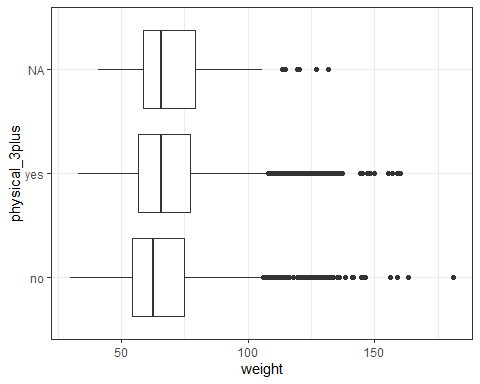
\includegraphics{Final_files/figure-latex/unnamed-chunk-9-1.pdf}

\begin{Shaded}
\begin{Highlighting}[]
\CommentTok{# scatterplot matrix for at least two of the independent variables and the dependent variable}
\NormalTok{train  }\OperatorTok
\StringTok{  }\KeywordTok{mutate}\NormalTok{(}\DataTypeTok{SalePrice.Adj =}\NormalTok{ SalePrice }\OperatorTok{/}\StringTok{ }\DecValTok{10000}\NormalTok{,}
         \DataTypeTok{GrLivArea.Adj =}\NormalTok{ GrLivArea }\OperatorTok{/}\StringTok{ }\DecValTok{100}\NormalTok{, }
         \DataTypeTok{LotArea.Adj =}\NormalTok{ LotArea }\OperatorTok{/}\StringTok{ }\DecValTok{100}\NormalTok{) }\OperatorTok\StringTok{ }
\StringTok{  }\NormalTok{dplyr}\OperatorTok{::}\KeywordTok{select}\NormalTok{(SalePrice.Adj, LotArea.Adj, LotFrontage, GrLivArea.Adj, TotalBsmtSF) }\OperatorTok
\StringTok{  }\KeywordTok{gather}\NormalTok{(variable, value, }\OperatorTok{-}\NormalTok{SalePrice.Adj) }\OperatorTok\StringTok{ }
\StringTok{  }\KeywordTok{ggplot}\NormalTok{(., }\KeywordTok{aes}\NormalTok{(value, SalePrice.Adj)) }\OperatorTok{+}\StringTok{ }
\StringTok{  }\KeywordTok{ggtitle}\NormalTok{(}\StringTok{"Some Interesting Independent Variables"}\NormalTok{) }\OperatorTok{+}\StringTok{ }
\StringTok{  }\KeywordTok{geom_point}\NormalTok{(}\DataTypeTok{fill =} \StringTok{"white"}\NormalTok{,}
             \DataTypeTok{size=}\DecValTok{1}\NormalTok{, }
             \DataTypeTok{shape=}\DecValTok{1}\NormalTok{, }
             \DataTypeTok{color=}\StringTok{"light blue"}\NormalTok{) }\OperatorTok{+}\StringTok{ }
\StringTok{  }\KeywordTok{geom_smooth}\NormalTok{(}\DataTypeTok{formula =}\NormalTok{ y}\OperatorTok{~}\NormalTok{x, }
              \DataTypeTok{method =} \StringTok{"lm"}\NormalTok{, }
              \DataTypeTok{size=}\NormalTok{.}\DecValTok{1}\NormalTok{,}
              \DataTypeTok{se =} \OtherTok{TRUE}\NormalTok{,}
              \DataTypeTok{color =} \StringTok{"black"}\NormalTok{, }
              \DataTypeTok{linetype =} \StringTok{"dotdash"}\NormalTok{, }
              \DataTypeTok{alpha=}\FloatTok{0.25}\NormalTok{) }\OperatorTok{+}\StringTok{ }
\StringTok{  }\KeywordTok{facet_wrap}\NormalTok{(}\OperatorTok{~}\NormalTok{variable, }
             \DataTypeTok{scales =}\StringTok{"free"}\NormalTok{,}
             \DataTypeTok{ncol =} \DecValTok{4}\NormalTok{)}
\end{Highlighting}
\end{Shaded}

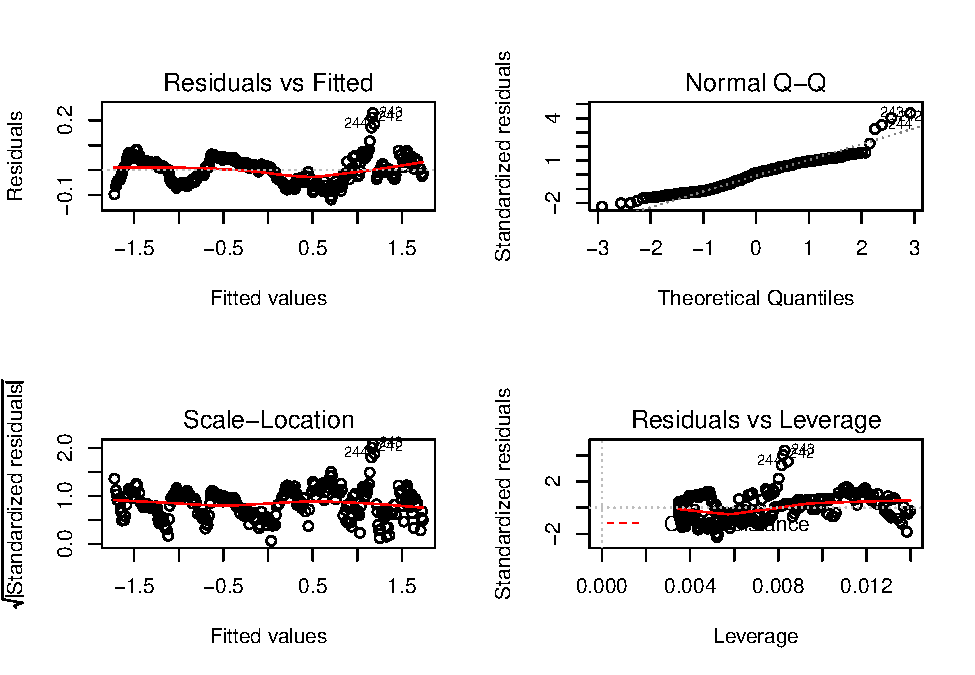
\includegraphics{Final_files/figure-latex/unnamed-chunk-10-1.pdf}

\begin{Shaded}
\begin{Highlighting}[]
  \CommentTok{# theme(axis.text.x = element_blank(), axis.text.y = element_blank())}
\end{Highlighting}
\end{Shaded}

\begin{Shaded}
\begin{Highlighting}[]
\NormalTok{train  }\OperatorTok
\StringTok{  }\KeywordTok{mutate}\NormalTok{(}\DataTypeTok{SalePrice.Adj =}\NormalTok{ SalePrice }\OperatorTok{/}\StringTok{ }\DecValTok{10000}\NormalTok{) }\OperatorTok\StringTok{ }
\StringTok{  }\NormalTok{dplyr}\OperatorTok{::}\KeywordTok{select}\NormalTok{(SalePrice.Adj, OverallQual, OverallCond, Neighborhood, BedroomAbvGr, FullBath, HalfBath) }\OperatorTok
\StringTok{  }\KeywordTok{gather}\NormalTok{(variable, value, }\OperatorTok{-}\NormalTok{SalePrice.Adj) }\OperatorTok\StringTok{ }
\StringTok{  }\KeywordTok{ggplot}\NormalTok{(., }\KeywordTok{aes}\NormalTok{(value, SalePrice.Adj)) }\OperatorTok{+}\StringTok{ }
\StringTok{  }\KeywordTok{ggtitle}\NormalTok{(}\StringTok{"Some Interesting Independent Variables"}\NormalTok{) }\OperatorTok{+}\StringTok{ }
\StringTok{  }\KeywordTok{geom_point}\NormalTok{(}\DataTypeTok{fill =} \StringTok{"white"}\NormalTok{,}
             \DataTypeTok{size=}\DecValTok{1}\NormalTok{, }
             \DataTypeTok{shape=}\DecValTok{1}\NormalTok{, }
             \DataTypeTok{color=}\StringTok{"light blue"}\NormalTok{) }\OperatorTok{+}\StringTok{ }
\StringTok{  }\KeywordTok{geom_smooth}\NormalTok{(}\DataTypeTok{formula =}\NormalTok{ y}\OperatorTok{~}\NormalTok{x, }
              \DataTypeTok{method =} \StringTok{"lm"}\NormalTok{, }
              \DataTypeTok{size=}\NormalTok{.}\DecValTok{1}\NormalTok{,}
              \DataTypeTok{se =} \OtherTok{TRUE}\NormalTok{,}
              \DataTypeTok{color =} \StringTok{"black"}\NormalTok{, }
              \DataTypeTok{linetype =} \StringTok{"dotdash"}\NormalTok{, }
              \DataTypeTok{alpha=}\FloatTok{0.25}\NormalTok{) }\OperatorTok{+}\StringTok{ }
\StringTok{  }\KeywordTok{facet_wrap}\NormalTok{(}\OperatorTok{~}\NormalTok{variable, }
             \DataTypeTok{scales =}\StringTok{"free"}\NormalTok{,}
             \DataTypeTok{ncol =} \DecValTok{4}\NormalTok{)}
\end{Highlighting}
\end{Shaded}

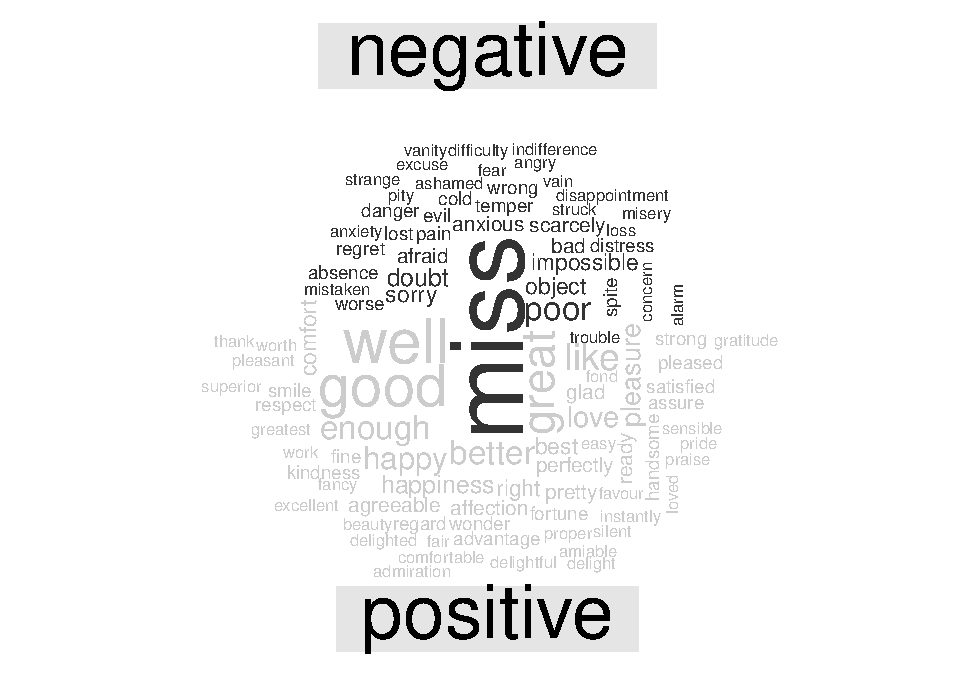
\includegraphics{Final_files/figure-latex/unnamed-chunk-11-1.pdf}

\begin{Shaded}
\begin{Highlighting}[]
\NormalTok{train  }\OperatorTok
\StringTok{  }\KeywordTok{mutate}\NormalTok{(}\DataTypeTok{SalePrice.Adj =}\NormalTok{ SalePrice }\OperatorTok{/}\StringTok{ }\DecValTok{10000}\NormalTok{, }
         \DataTypeTok{GrLivArea.Adj =}\NormalTok{ GrLivArea }\OperatorTok{/}\StringTok{ }\DecValTok{100}\NormalTok{, }
         \DataTypeTok{LotArea.Adj =}\NormalTok{ LotArea }\OperatorTok{/}\StringTok{ }\DecValTok{100}\NormalTok{) }\OperatorTok\StringTok{ }
\StringTok{  }\NormalTok{dplyr}\OperatorTok{::}\KeywordTok{select}\NormalTok{(SalePrice.Adj, OverallQual, OverallCond, Neighborhood, BedroomAbvGr, FullBath, HalfBath, }
\NormalTok{         LotArea.Adj, LotFrontage, GrLivArea.Adj, TotalBsmtSF) }\OperatorTok
\StringTok{  }\KeywordTok{gather}\NormalTok{(variable, value) }\OperatorTok\StringTok{ }
\StringTok{  }\KeywordTok{ggplot}\NormalTok{(., }\KeywordTok{aes}\NormalTok{(value)) }\OperatorTok{+}\StringTok{ }
\StringTok{  }\KeywordTok{ggtitle}\NormalTok{(}\StringTok{"Distribution of Interesting Independent Variables"}\NormalTok{) }\OperatorTok{+}\StringTok{ }
\StringTok{  }\KeywordTok{geom_histogram}\NormalTok{(}\DataTypeTok{fill =} \StringTok{"white"}\NormalTok{,}
             \DataTypeTok{size=}\DecValTok{1}\NormalTok{, }
             \DataTypeTok{shape=}\DecValTok{1}\NormalTok{, }
             \DataTypeTok{color=}\StringTok{"light blue"}\NormalTok{, }
             \DataTypeTok{stat =} \StringTok{"count"}\NormalTok{) }\OperatorTok{+}\StringTok{ }
\StringTok{  }\KeywordTok{theme}\NormalTok{(}\DataTypeTok{axis.text.x =} \KeywordTok{element_blank}\NormalTok{()) }\OperatorTok{+}\StringTok{ }
\StringTok{  }\KeywordTok{facet_wrap}\NormalTok{(}\OperatorTok{~}\NormalTok{variable, }
             \DataTypeTok{scales =}\StringTok{"free"}\NormalTok{,}
             \DataTypeTok{ncol =} \DecValTok{4}\NormalTok{)}
\end{Highlighting}
\end{Shaded}

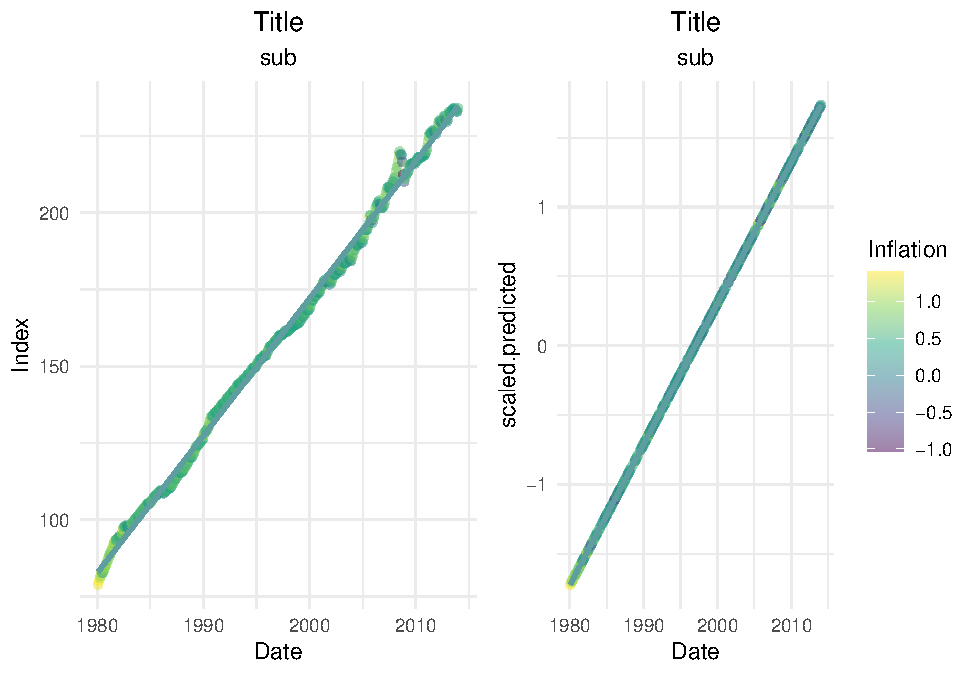
\includegraphics{Final_files/figure-latex/unnamed-chunk-12-1.pdf}

\begin{Shaded}
\begin{Highlighting}[]
\NormalTok{train  }\OperatorTok
\StringTok{  }\KeywordTok{mutate}\NormalTok{(}\DataTypeTok{SalePrice.Adj =}\NormalTok{ SalePrice }\OperatorTok{/}\StringTok{ }\DecValTok{10000}\NormalTok{, }
         \DataTypeTok{GrLivArea.Adj =}\NormalTok{ GrLivArea }\OperatorTok{/}\StringTok{ }\DecValTok{100}\NormalTok{, }
         \DataTypeTok{LotArea.Adj =}\NormalTok{ LotArea }\OperatorTok{/}\StringTok{ }\DecValTok{100}\NormalTok{) }\OperatorTok\StringTok{ }
\StringTok{  }\NormalTok{dplyr}\OperatorTok{::}\KeywordTok{select}\NormalTok{(SalePrice.Adj, OverallQual, OverallCond, Neighborhood, BedroomAbvGr, FullBath, HalfBath, }
\NormalTok{         LotArea.Adj, LotFrontage, GrLivArea.Adj, TotalBsmtSF) }\OperatorTok
\StringTok{  }\KeywordTok{gather}\NormalTok{(variable, value) }\OperatorTok\StringTok{ }
\StringTok{  }\KeywordTok{ggplot}\NormalTok{(., }\KeywordTok{aes}\NormalTok{(value)) }\OperatorTok{+}\StringTok{ }
\StringTok{  }\KeywordTok{ggtitle}\NormalTok{(}\StringTok{"Distribution of Interesting Independent Variables"}\NormalTok{) }\OperatorTok{+}\StringTok{ }
\StringTok{  }\KeywordTok{geom_density}\NormalTok{(}\DataTypeTok{fill =} \StringTok{"white"}\NormalTok{,}
             \DataTypeTok{size=}\DecValTok{1}\NormalTok{, }
             \DataTypeTok{shape=}\DecValTok{1}\NormalTok{, }
             \DataTypeTok{color=}\StringTok{"light blue"}\NormalTok{) }\OperatorTok{+}\StringTok{ }
\StringTok{  }\KeywordTok{theme}\NormalTok{(}\DataTypeTok{axis.text.x =} \KeywordTok{element_blank}\NormalTok{()) }\OperatorTok{+}\StringTok{ }
\StringTok{  }\KeywordTok{facet_wrap}\NormalTok{(}\OperatorTok{~}\NormalTok{variable, }
             \DataTypeTok{scales =}\StringTok{"free"}\NormalTok{,}
             \DataTypeTok{ncol =} \DecValTok{4}\NormalTok{)}
\end{Highlighting}
\end{Shaded}

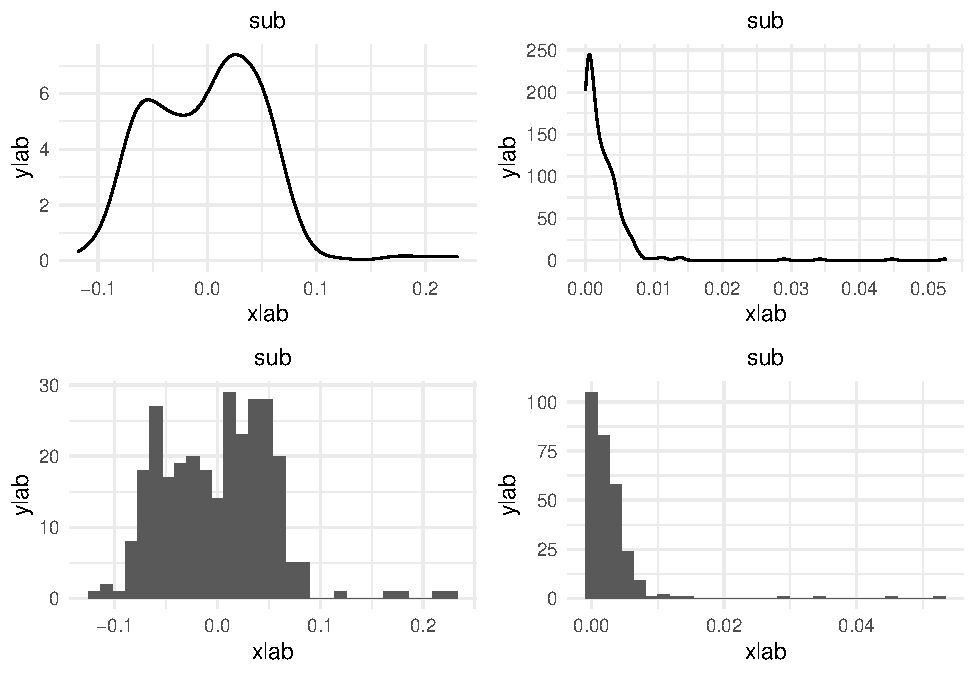
\includegraphics{Final_files/figure-latex/unnamed-chunk-13-1.pdf}

\begin{Shaded}
\begin{Highlighting}[]
\CommentTok{# Derive a correlation matrix for any three quantitative variables}
\NormalTok{train }\OperatorTok\StringTok{ }
\StringTok{  }\NormalTok{dplyr}\OperatorTok{::}\KeywordTok{select}\NormalTok{(SalePrice, LotArea, OverallQual, OverallCond) }\OperatorTok\StringTok{ }
\StringTok{  }\KeywordTok{cor}\NormalTok{() }\OperatorTok\StringTok{ }
\StringTok{  }\KeywordTok{as.matrix}\NormalTok{()}
\end{Highlighting}
\end{Shaded}

\begin{verbatim}
##               SalePrice     LotArea OverallQual OverallCond
## SalePrice    1.00000000  0.26384335  0.79098160 -0.07785589
## LotArea      0.26384335  1.00000000  0.10580574 -0.00563627
## OverallQual  0.79098160  0.10580574  1.00000000 -0.09193234
## OverallCond -0.07785589 -0.00563627 -0.09193234  1.00000000
\end{verbatim}

\begin{Shaded}
\begin{Highlighting}[]
\KeywordTok{cor.test}\NormalTok{(train}\OperatorTok{$}\NormalTok{SalePrice, train}\OperatorTok{$}\NormalTok{OverallCond, }\DataTypeTok{conf.level =} \FloatTok{0.80}\NormalTok{)}
\end{Highlighting}
\end{Shaded}

\begin{verbatim}
## 
##  Pearson's product-moment correlation
## 
## data:  train$SalePrice and train$OverallCond
## t = -2.9819, df = 1458, p-value = 0.002912
## alternative hypothesis: true correlation is not equal to 0
## 80 percent confidence interval:
##  -0.1111272 -0.0444103
## sample estimates:
##         cor 
## -0.07785589
\end{verbatim}

\begin{Shaded}
\begin{Highlighting}[]
\KeywordTok{cor.test}\NormalTok{(train}\OperatorTok{$}\NormalTok{SalePrice, train}\OperatorTok{$}\NormalTok{OverallQual, }\DataTypeTok{conf.level =} \FloatTok{0.80}\NormalTok{)}
\end{Highlighting}
\end{Shaded}

\begin{verbatim}
## 
##  Pearson's product-moment correlation
## 
## data:  train$SalePrice and train$OverallQual
## t = 49.364, df = 1458, p-value < 2.2e-16
## alternative hypothesis: true correlation is not equal to 0
## 80 percent confidence interval:
##  0.7780752 0.8032204
## sample estimates:
##       cor 
## 0.7909816
\end{verbatim}

\begin{Shaded}
\begin{Highlighting}[]
\KeywordTok{cor.test}\NormalTok{(train}\OperatorTok{$}\NormalTok{SalePrice, train}\OperatorTok{$}\NormalTok{LotArea, }\DataTypeTok{conf.level =} \FloatTok{0.80}\NormalTok{)}
\end{Highlighting}
\end{Shaded}

\begin{verbatim}
## 
##  Pearson's product-moment correlation
## 
## data:  train$SalePrice and train$LotArea
## t = 10.445, df = 1458, p-value < 2.2e-16
## alternative hypothesis: true correlation is not equal to 0
## 80 percent confidence interval:
##  0.2323391 0.2947946
## sample estimates:
##       cor 
## 0.2638434
\end{verbatim}

There should be no worries about familywise errors which is the
probability of making a false discovery (in other words, type 1 errors)
because the values are relatively intuitive and easily interpreted as
right or wrong. For example, a false rejection of the null hypothesis in
the case of LotArea would likely mean that we conclude that greater lot
sizes did not have an effect on sale price when we know this to be
false. We should expect that for almost any of these variables an
increase in something considered good or valuable by most people would
result in an increase in sales price.

Meanwhile our variables could use some help and it is doubtful that many
are beneficial to use in predicting sales price. In some of the most
interesting variables that we thought would have the most influence over
sales price, many are right skewed heavily. This will cause the model to
predict higher than observed values if not accounted for.

The three variables we expect to perform best are LotArea, OverallQual,
and OverallCond. Their correlations are completely different.
OverallQual had the strongest correlation with SalePrice at about 0.79
which makes sense given that most people would consider it important to
think about the overall quality of the home before agreeing to purchase
it. However, there is still plenty of room for misinterpretation in any
of these variables.

\hypertarget{section-2-linear-algebra-and-correlation}{%
\subsubsection{Section 2: Linear Algebra and
Correlation}\label{section-2-linear-algebra-and-correlation}}

\begin{Shaded}
\begin{Highlighting}[]
\NormalTok{cor.mtx <-}\StringTok{ }\NormalTok{train }\OperatorTok\StringTok{ }
\StringTok{  }\NormalTok{dplyr}\OperatorTok{::}\KeywordTok{select}\NormalTok{(SalePrice, LotArea, OverallQual, OverallCond) }\OperatorTok\StringTok{ }
\StringTok{  }\KeywordTok{cor}\NormalTok{() }\OperatorTok\StringTok{ }
\StringTok{  }\KeywordTok{as.matrix}\NormalTok{()}
\NormalTok{pcn.mtx <-}\StringTok{ }\KeywordTok{solve}\NormalTok{(cor.mtx)}
\NormalTok{rdu.mtx <-}\StringTok{ }\NormalTok{cor.mtx }\OperatorTok\StringTok{ }\NormalTok{pcn.mtx}
\NormalTok{lud.mtx <-}\StringTok{ }\KeywordTok{lu.decomposition}\NormalTok{(rdu.mtx)}
\NormalTok{cor.mtx}
\end{Highlighting}
\end{Shaded}

\begin{verbatim}
##               SalePrice     LotArea OverallQual OverallCond
## SalePrice    1.00000000  0.26384335  0.79098160 -0.07785589
## LotArea      0.26384335  1.00000000  0.10580574 -0.00563627
## OverallQual  0.79098160  0.10580574  1.00000000 -0.09193234
## OverallCond -0.07785589 -0.00563627 -0.09193234  1.00000000
\end{verbatim}

\begin{Shaded}
\begin{Highlighting}[]
\NormalTok{pcn.mtx}
\end{Highlighting}
\end{Shaded}

\begin{verbatim}
##               SalePrice      LotArea OverallQual  OverallCond
## SalePrice    2.92833783 -0.533593316  -2.2582064  0.017378675
## LotArea     -0.53359332  1.108568702   0.3040949 -0.007339038
## OverallQual -2.25820645  0.304094866   2.7613570  0.079757301
## OverallCond  0.01737868 -0.007339038   0.0797573  1.008643943
\end{verbatim}

\begin{Shaded}
\begin{Highlighting}[]
\NormalTok{rdu.mtx}
\end{Highlighting}
\end{Shaded}

\begin{verbatim}
##                 SalePrice       LotArea   OverallQual   OverallCond
## SalePrice    1.000000e+00  2.287667e-17  8.673617e-19  0.000000e+00
## LotArea     -2.535678e-17  1.000000e+00 -6.342583e-18 -8.673617e-19
## OverallQual -1.084202e-16  1.821460e-17  1.000000e+00  0.000000e+00
## OverallCond -1.734723e-17 -6.938894e-18  4.163336e-17  1.000000e+00
\end{verbatim}

\begin{Shaded}
\begin{Highlighting}[]
\NormalTok{lud.mtx}
\end{Highlighting}
\end{Shaded}

\begin{verbatim}
## $L
##               [,1]          [,2]         [,3] [,4]
## [1,]  1.000000e+00  0.000000e+00 0.000000e+00    0
## [2,] -2.535678e-17  1.000000e+00 0.000000e+00    0
## [3,] -1.084202e-16  1.821460e-17 1.000000e+00    0
## [4,] -1.734723e-17 -6.938894e-18 4.163336e-17    1
## 
## $U
##      [,1]         [,2]          [,3]          [,4]
## [1,]    1 2.287667e-17  8.673617e-19  0.000000e+00
## [2,]    0 1.000000e+00 -6.342583e-18 -8.673617e-19
## [3,]    0 0.000000e+00  1.000000e+00  1.579864e-35
## [4,]    0 0.000000e+00  0.000000e+00  1.000000e+00
\end{verbatim}

\hypertarget{section-3-calculus-based-probability-statistics}{%
\subsubsection{Section 3: Calculus-Based Probability \&
Statistics}\label{section-3-calculus-based-probability-statistics}}

\begin{Shaded}
\begin{Highlighting}[]
\NormalTok{fd.exp <-}\StringTok{ }\KeywordTok{fitdistr}\NormalTok{(train}\OperatorTok{$}\NormalTok{LotArea, }\DataTypeTok{densfun =} \StringTok{"exponential"}\NormalTok{)}
\NormalTok{y <-}\StringTok{ }\NormalTok{fd.exp}\OperatorTok{$}\NormalTok{estimate}
\NormalTok{rate <-}\StringTok{ }\DecValTok{1}\OperatorTok{/}\NormalTok{y}
\NormalTok{n <-}\StringTok{ }\KeywordTok{rexp}\NormalTok{(}\DecValTok{1000}\NormalTok{, rate)}
\KeywordTok{par}\NormalTok{(}\DataTypeTok{mfrow =} \KeywordTok{c}\NormalTok{(}\DecValTok{1}\NormalTok{,}\DecValTok{2}\NormalTok{))}
\KeywordTok{hist}\NormalTok{(train}\OperatorTok{$}\NormalTok{LotArea, }\DataTypeTok{breaks =} \DecValTok{75}\NormalTok{, }\DataTypeTok{main =} \StringTok{"Origional"}\NormalTok{)}
\KeywordTok{hist}\NormalTok{(n, }\DataTypeTok{breaks =} \DecValTok{75}\NormalTok{, }\DataTypeTok{main =} \StringTok{"Exponential"}\NormalTok{)}
\end{Highlighting}
\end{Shaded}

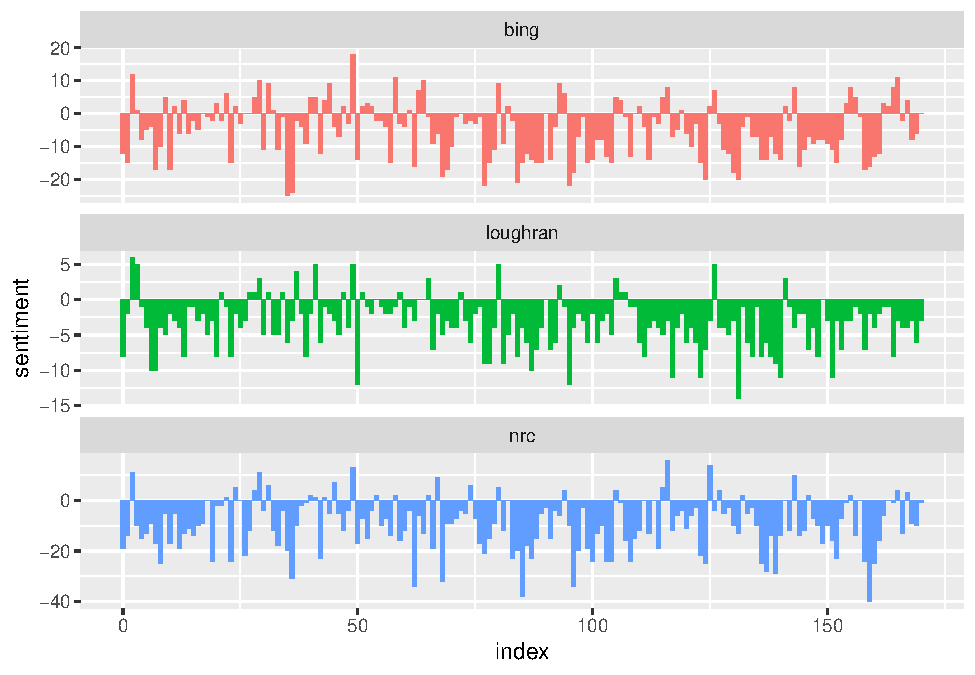
\includegraphics{Final_files/figure-latex/unnamed-chunk-17-1.pdf}

\begin{Shaded}
\begin{Highlighting}[]
\CommentTok{# 5th and 95th Percentiles }
\KeywordTok{print}\NormalTok{(}\KeywordTok{paste}\NormalTok{(}\StringTok{"CDF Percentile ="}\NormalTok{, }\KeywordTok{signif}\NormalTok{(}\KeywordTok{qexp}\NormalTok{(}\KeywordTok{c}\NormalTok{(}\FloatTok{0.05}\NormalTok{, }\FloatTok{0.95}\NormalTok{), }\DataTypeTok{rate =}\NormalTok{ rate), }\DecValTok{3}\NormalTok{)))}
\end{Highlighting}
\end{Shaded}

\begin{verbatim}
## [1] "CDF Percentile = 4.88e-06" "CDF Percentile = 0.000285"
\end{verbatim}

\begin{Shaded}
\begin{Highlighting}[]
\CommentTok{# 95% confidence interval }
\KeywordTok{print}\NormalTok{(}\KeywordTok{paste}\NormalTok{(}\StringTok{"95% Confidence ="}\NormalTok{,}\KeywordTok{round}\NormalTok{((}\KeywordTok{qnorm}\NormalTok{(}\KeywordTok{c}\NormalTok{(}\FloatTok{0.025}\NormalTok{, }\FloatTok{0.975}\NormalTok{),}
      \DataTypeTok{mean=}\KeywordTok{mean}\NormalTok{(train}\OperatorTok{$}\NormalTok{LotArea), }\DataTypeTok{sd=}\KeywordTok{sd}\NormalTok{(train}\OperatorTok{$}\NormalTok{LotArea))), }\DecValTok{3}\NormalTok{)))}
\end{Highlighting}
\end{Shaded}

\begin{verbatim}
## [1] "95% Confidence = -9046.092" "95% Confidence = 30079.748"
\end{verbatim}

\begin{Shaded}
\begin{Highlighting}[]
\KeywordTok{print}\NormalTok{(}\KeywordTok{paste}\NormalTok{(}\StringTok{"Empirical ="}\NormalTok{, }\KeywordTok{round}\NormalTok{(}\KeywordTok{quantile}\NormalTok{(train}\OperatorTok{$}\NormalTok{LotArea, }\KeywordTok{c}\NormalTok{(}\FloatTok{0.05}\NormalTok{, }\FloatTok{0.95}\NormalTok{)), }\DecValTok{3}\NormalTok{)))}
\end{Highlighting}
\end{Shaded}

\begin{verbatim}
## [1] "Empirical = 3311.7"   "Empirical = 17401.15"
\end{verbatim}

The 5th and 95th percentiles differ from CDF to Empirical. Our histogram
shows the exponential distribution spreads itself more normally than the
original. From the 95\% confidence calculation we have the range
-9046.092 to 30079.748. This is completely unrealistic of the variable
given that lot area is not normally distributed and is also always
positive (otherwise you have nothing to sell). Alternatively we have the
empirically calculated range 3311.7 to 17401.15 which is larger but more
realistic.

\hypertarget{section-4-modeling}{%
\subsubsection{Section 4: Modeling}\label{section-4-modeling}}

\begin{Shaded}
\begin{Highlighting}[]
\NormalTok{mod1 <-}\StringTok{ }\KeywordTok{lm}\NormalTok{(SalePrice}\OperatorTok{~}\NormalTok{LotArea }\OperatorTok{+}\StringTok{ }\NormalTok{OverallQual, train)}
\KeywordTok{summary}\NormalTok{(mod1)}
\end{Highlighting}
\end{Shaded}

\begin{verbatim}
## 
## Call:
## lm(formula = SalePrice ~ LotArea + OverallQual, data = train)
## 
## Residuals:
##     Min      1Q  Median      3Q     Max 
## -271225  -26819   -1459   20172  385190 
## 
## Coefficients:
##               Estimate Std. Error t value Pr(>|t|)    
## (Intercept) -1.047e+05  5.547e+03  -18.88   <2e-16 ***
## LotArea      1.450e+00  1.225e-01   11.83   <2e-16 ***
## OverallQual  4.433e+04  8.844e+02   50.12   <2e-16 ***
## ---
## Signif. codes:  0 '***' 0.001 '**' 0.01 '*' 0.05 '.' 0.1 ' ' 1
## 
## Residual standard error: 46460 on 1457 degrees of freedom
## Multiple R-squared:  0.6585, Adjusted R-squared:  0.658 
## F-statistic:  1405 on 2 and 1457 DF,  p-value: < 2.2e-16
\end{verbatim}

\begin{Shaded}
\begin{Highlighting}[]
\KeywordTok{par}\NormalTok{(}\DataTypeTok{mfrow =} \KeywordTok{c}\NormalTok{(}\DecValTok{2}\NormalTok{,}\DecValTok{2}\NormalTok{))}
\KeywordTok{plot}\NormalTok{(mod1)}
\end{Highlighting}
\end{Shaded}

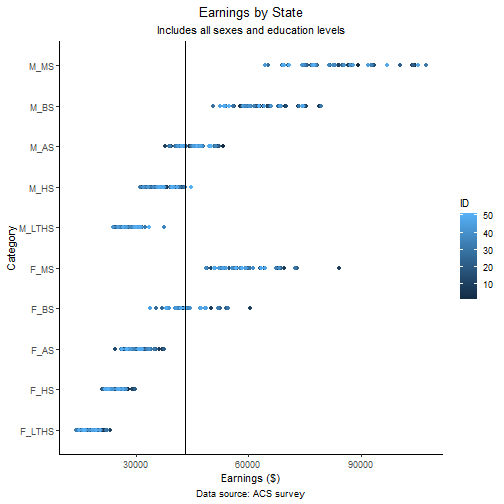
\includegraphics{Final_files/figure-latex/unnamed-chunk-19-1.pdf}

This model was meant to elucidate the behavior of two of the most likely
variables thought to influence sales price. Of course, this could be
improved since we have plenty of room to do so. Ignoring the problem
outliers in our Residuals vs Leverage plot as well as the sinking
Scale-Location plot, we have close enough to normal set to build on
(though declaring it normal is a stretch here too given the tails).
Interestingly, our \(R^2\) is moderately strong at about 0.659.

\begin{Shaded}
\begin{Highlighting}[]
\NormalTok{mod2.lm <-}\StringTok{ }\KeywordTok{lm}\NormalTok{(SalePrice }\OperatorTok{~}\StringTok{ }\NormalTok{LotArea }\OperatorTok{+}\StringTok{ }
\StringTok{                }\NormalTok{Neighborhood }\OperatorTok{+}\StringTok{ }
\StringTok{                }\NormalTok{LotFrontage }\OperatorTok{+}\StringTok{ }
\StringTok{                }\NormalTok{OverallQual }\OperatorTok{+}\StringTok{ }
\StringTok{                }\NormalTok{OverallCond }\OperatorTok{+}\StringTok{ }
\StringTok{                }\NormalTok{GrLivArea }\OperatorTok{+}\StringTok{ }
\StringTok{                }\NormalTok{HalfBath }\OperatorTok{+}\StringTok{ }
\StringTok{                }\NormalTok{FullBath }\OperatorTok{+}\StringTok{ }
\StringTok{                }\NormalTok{TotRmsAbvGrd }\OperatorTok{+}\StringTok{ }
\StringTok{                }\NormalTok{TotalBsmtSF }\OperatorTok{+}\StringTok{ }
\StringTok{                }\NormalTok{YearRemodAdd }\OperatorTok{+}\StringTok{ }
\StringTok{                }\NormalTok{YearBuilt }\OperatorTok{+}\StringTok{ }
\StringTok{                }\NormalTok{Fireplaces }\OperatorTok{+}\StringTok{ }
\StringTok{                }\NormalTok{GarageFinish }\OperatorTok{+}\StringTok{ }
\StringTok{                }\NormalTok{PavedDrive }\OperatorTok{+}\StringTok{ }
\StringTok{                }\NormalTok{GarageArea }\OperatorTok{+}\StringTok{ }
\StringTok{                }\NormalTok{GarageYrBlt }\OperatorTok{+}
\StringTok{                }\NormalTok{GarageCars }\OperatorTok{+}\StringTok{ }
\StringTok{                }\NormalTok{PoolArea }\OperatorTok{+}\StringTok{ }
\StringTok{                }\NormalTok{KitchenAbvGr }\OperatorTok{+}\StringTok{ }
\StringTok{                }\NormalTok{KitchenQual }\OperatorTok{+}\StringTok{ }
\StringTok{                }\NormalTok{SaleCondition }\OperatorTok{+}\StringTok{ }
\StringTok{                }\NormalTok{SaleType }\OperatorTok{+}
\StringTok{                }\KeywordTok{factor}\NormalTok{(OverallQual) }\OperatorTok{+}\StringTok{ }
\StringTok{                }\NormalTok{LandSlope }\OperatorTok{+}\StringTok{ }
\StringTok{                }\KeywordTok{rexp}\NormalTok{(LotArea) }\OperatorTok{+}
\StringTok{                }\KeywordTok{rexp}\NormalTok{(LotFrontage) }\OperatorTok{+}\StringTok{ }
\StringTok{                }\KeywordTok{rexp}\NormalTok{(GrLivArea) }\OperatorTok{+}\StringTok{ }
\StringTok{                }\KeywordTok{rexp}\NormalTok{(TotRmsAbvGrd) }\OperatorTok{+}\StringTok{ }
\StringTok{                }\KeywordTok{rexp}\NormalTok{(TotalBsmtSF) }\OperatorTok{+}
\StringTok{                }\KeywordTok{rexp}\NormalTok{(GarageArea) }
\NormalTok{              , train)}
\NormalTok{mod2.both <-}\StringTok{ }\KeywordTok{stepAIC}\NormalTok{(mod2.lm, }\DataTypeTok{trace =}\NormalTok{ F, }\DataTypeTok{direction =} \StringTok{"both"}\NormalTok{)}
\NormalTok{mod2.call <-}\StringTok{ }\KeywordTok{summary}\NormalTok{(mod2.both)}\OperatorTok{$}\NormalTok{call}
\NormalTok{mod2 <-}\StringTok{ }\KeywordTok{lm}\NormalTok{(mod2.call[}\DecValTok{2}\NormalTok{], train)}
\KeywordTok{summary}\NormalTok{(mod2)}
\end{Highlighting}
\end{Shaded}

\begin{verbatim}
## 
## Call:
## lm(formula = mod2.call[2], data = train)
## 
## Residuals:
##     Min      1Q  Median      3Q     Max 
## -393429  -12267    -636   10598  238004 
## 
## Coefficients:
##                         Estimate Std. Error t value Pr(>|t|)    
## (Intercept)           -4.709e+05  2.225e+05  -2.117 0.034530 *  
## LotArea                7.709e-01  1.585e-01   4.864 1.32e-06 ***
## NeighborhoodBlueste   -1.355e+04  2.492e+04  -0.544 0.586707    
## NeighborhoodBrDale    -7.978e+02  1.323e+04  -0.060 0.951921    
## NeighborhoodBrkSide    1.483e+04  1.171e+04   1.267 0.205491    
## NeighborhoodClearCr    2.964e+04  1.372e+04   2.160 0.031006 *  
## NeighborhoodCollgCr    2.517e+04  9.649e+03   2.609 0.009221 ** 
## NeighborhoodCrawfor    3.690e+04  1.150e+04   3.210 0.001366 ** 
## NeighborhoodEdwards   -5.310e+03  1.059e+04  -0.502 0.615997    
## NeighborhoodGilbert    1.195e+04  1.033e+04   1.157 0.247640    
## NeighborhoodIDOTRR     1.430e+03  1.253e+04   0.114 0.909138    
## NeighborhoodMeadowV   -8.362e+03  1.429e+04  -0.585 0.558630    
## NeighborhoodMitchel    1.885e+04  1.116e+04   1.690 0.091391 .  
## NeighborhoodNAmes      1.583e+04  1.026e+04   1.542 0.123390    
## NeighborhoodNoRidge    7.785e+04  1.127e+04   6.909 8.44e-12 ***
## NeighborhoodNPkVill    8.952e+02  1.581e+04   0.057 0.954861    
## NeighborhoodNridgHt    4.630e+04  1.019e+04   4.543 6.17e-06 ***
## NeighborhoodNWAmes     1.240e+04  1.077e+04   1.151 0.249932    
## NeighborhoodOldTown    4.527e+03  1.129e+04   0.401 0.688593    
## NeighborhoodSawyer     1.382e+04  1.096e+04   1.261 0.207736    
## NeighborhoodSawyerW    2.367e+04  1.051e+04   2.252 0.024505 *  
## NeighborhoodSomerst    2.739e+04  9.918e+03   2.762 0.005848 ** 
## NeighborhoodStoneBr    6.889e+04  1.181e+04   5.834 7.19e-09 ***
## NeighborhoodSWISU      4.196e+03  1.320e+04   0.318 0.750622    
## NeighborhoodTimber     2.584e+04  1.098e+04   2.354 0.018740 *  
## NeighborhoodVeenker    4.400e+04  1.564e+04   2.814 0.004985 ** 
## LotFrontage           -1.206e+02  5.472e+01  -2.204 0.027729 *  
## OverallCond            7.554e+03  1.241e+03   6.085 1.63e-09 ***
## GrLivArea              3.687e+01  5.250e+00   7.023 3.87e-12 ***
## HalfBath               1.307e+02  2.759e+03   0.047 0.962237    
## FullBath               3.918e+03  3.243e+03   1.208 0.227192    
## TotRmsAbvGrd           2.368e+03  1.234e+03   1.918 0.055333 .  
## TotalBsmtSF            1.368e+01  3.421e+00   3.998 6.84e-05 ***
## YearRemodAdd           5.593e+01  8.245e+01   0.678 0.497701    
## YearBuilt              2.956e+02  9.604e+01   3.077 0.002143 ** 
## Fireplaces             7.827e+03  1.983e+03   3.947 8.42e-05 ***
## GarageFinishRFn       -3.869e+03  3.001e+03  -1.289 0.197550    
## GarageFinishUnf       -9.218e+03  3.443e+03  -2.677 0.007535 ** 
## PavedDriveP           -3.176e+03  8.484e+03  -0.374 0.708224    
## PavedDriveY            4.211e+03  5.390e+03   0.781 0.434887    
## GarageArea            -7.639e-01  1.127e+01  -0.068 0.945959    
## GarageYrBlt           -9.415e+01  8.146e+01  -1.156 0.248014    
## GarageCars             1.460e+04  3.203e+03   4.559 5.73e-06 ***
## PoolArea              -3.694e+01  2.608e+01  -1.417 0.156917    
## KitchenAbvGr          -2.944e+04  5.827e+03  -5.053 5.12e-07 ***
## KitchenQualFa         -2.673e+04  9.319e+03  -2.869 0.004204 ** 
## KitchenQualGd         -2.104e+04  4.995e+03  -4.213 2.74e-05 ***
## KitchenQualTA         -2.412e+04  5.709e+03  -4.224 2.60e-05 ***
## SaleConditionAdjLand   4.215e+04  3.364e+04   1.253 0.210525    
## SaleConditionAlloca    3.930e+03  1.242e+04   0.316 0.751776    
## SaleConditionFamily   -4.294e+03  8.764e+03  -0.490 0.624290    
## SaleConditionNormal    5.163e+03  4.154e+03   1.243 0.214179    
## SaleConditionPartial   1.988e+04  5.468e+03   3.636 0.000290 ***
## factor(OverallQual)3  -4.118e+02  2.573e+04  -0.016 0.987235    
## factor(OverallQual)4  -3.055e+03  2.405e+04  -0.127 0.898929    
## factor(OverallQual)5  -2.315e+03  2.401e+04  -0.096 0.923197    
## factor(OverallQual)6  -1.447e+03  2.411e+04  -0.060 0.952159    
## factor(OverallQual)7   8.881e+03  2.436e+04   0.365 0.715461    
## factor(OverallQual)8   3.192e+04  2.471e+04   1.292 0.196624    
## factor(OverallQual)9   8.513e+04  2.552e+04   3.335 0.000882 ***
## factor(OverallQual)10  1.077e+05  2.681e+04   4.018 6.28e-05 ***
## LandSlopeMod           1.320e+04  5.332e+03   2.476 0.013447 *  
## LandSlopeSev          -2.185e+04  1.712e+04  -1.277 0.202047    
## rexp(LotArea)         -6.386e+02  9.900e+02  -0.645 0.519025    
## rexp(LotFrontage)      1.267e+02  1.066e+03   0.119 0.905379    
## rexp(GrLivArea)        7.868e+02  9.221e+02   0.853 0.393733    
## rexp(TotRmsAbvGrd)    -3.576e+02  1.025e+03  -0.349 0.727288    
## rexp(TotalBsmtSF)      2.712e+02  9.621e+02   0.282 0.778076    
## rexp(GarageArea)      -8.183e+02  9.876e+02  -0.829 0.407503    
## ---
## Signif. codes:  0 '***' 0.001 '**' 0.01 '*' 0.05 '.' 0.1 ' ' 1
## 
## Residual standard error: 32160 on 1058 degrees of freedom
##   (333 observations deleted due to missingness)
## Multiple R-squared:  0.8597, Adjusted R-squared:  0.8507 
## F-statistic: 95.32 on 68 and 1058 DF,  p-value: < 2.2e-16
\end{verbatim}

\begin{Shaded}
\begin{Highlighting}[]
\KeywordTok{plot}\NormalTok{(mod2)}
\end{Highlighting}
\end{Shaded}

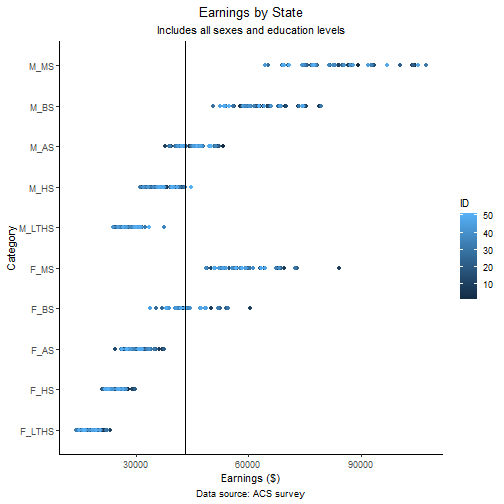
\includegraphics{Final_files/figure-latex/unnamed-chunk-20-1.pdf}
\includegraphics{Final_files/figure-latex/unnamed-chunk-20-2.pdf}
\includegraphics{Final_files/figure-latex/unnamed-chunk-20-3.pdf}
\includegraphics{Final_files/figure-latex/unnamed-chunk-20-4.pdf}

The goal in this model was to add any variables to the plot we thougth
might influence the sales price at then see if there any new trends we
to be noticed and there are. Our initial expectation is at least
partially wrong. We missed out on several beneficial variables (and may
have missed more than what is listed here). Many of these predictors are
not significant or particularly useful in predicting sales price. We
select those that are significant and clean them up a bit before
creating our third model.

\begin{Shaded}
\begin{Highlighting}[]
\NormalTok{train}\OperatorTok{$}\NormalTok{LotFrontage[}\KeywordTok{is.na}\NormalTok{(train}\OperatorTok{$}\NormalTok{LotFrontage)] <-}\StringTok{ }\KeywordTok{median}\NormalTok{(train}\OperatorTok{$}\NormalTok{LotFrontage, }\DataTypeTok{na.rm =}\NormalTok{ T)}
\NormalTok{train}\OperatorTok{$}\NormalTok{GarageCars[}\KeywordTok{is.na}\NormalTok{(train}\OperatorTok{$}\NormalTok{GarageCars)] <-}\StringTok{ }\KeywordTok{median}\NormalTok{(train}\OperatorTok{$}\NormalTok{GarageCars, }\DataTypeTok{na.rm =}\NormalTok{ T)}
\NormalTok{train}\OperatorTok{$}\NormalTok{TotalBsmtSF[}\KeywordTok{is.na}\NormalTok{(train}\OperatorTok{$}\NormalTok{TotalBsmtSF)] <-}\StringTok{ }\KeywordTok{median}\NormalTok{(train}\OperatorTok{$}\NormalTok{TotalBsmtSF, }\DataTypeTok{na.rm =}\NormalTok{ T)}
\NormalTok{train}\OperatorTok{$}\NormalTok{SaleType[}\KeywordTok{is.na}\NormalTok{(train}\OperatorTok{$}\NormalTok{SaleType)] <-}\StringTok{ "WD"}
\NormalTok{train}\OperatorTok{$}\NormalTok{KitchenQual[}\KeywordTok{is.na}\NormalTok{(train}\OperatorTok{$}\NormalTok{KitchenQual)] <-}\StringTok{ "TA"}
\NormalTok{train}\OperatorTok{$}\NormalTok{GarageFinish[}\KeywordTok{is.na}\NormalTok{(train}\OperatorTok{$}\NormalTok{GarageFinish)] <-}\StringTok{ "Unf"}
\NormalTok{mod3 <-}\StringTok{ }\KeywordTok{lm}\NormalTok{(SalePrice }\OperatorTok{~}\StringTok{ }
\StringTok{             }\NormalTok{LandSlope }\OperatorTok{+}\StringTok{ }
\StringTok{             }\NormalTok{OverallQual }\OperatorTok{+}\StringTok{ }
\StringTok{             }\NormalTok{KitchenQual }\OperatorTok{+}\StringTok{ }
\StringTok{             }\NormalTok{KitchenAbvGr }\OperatorTok{+}\StringTok{ }
\StringTok{             }\NormalTok{GarageCars }\OperatorTok{+}\StringTok{ }
\StringTok{             }\NormalTok{GarageFinish }\OperatorTok{+}\StringTok{ }
\StringTok{             }\NormalTok{Fireplaces }\OperatorTok{+}\StringTok{ }
\StringTok{             }\NormalTok{YearBuilt }\OperatorTok{+}\StringTok{ }
\StringTok{             }\NormalTok{TotalBsmtSF }\OperatorTok{+}\StringTok{ }
\StringTok{             }\NormalTok{TotRmsAbvGrd }\OperatorTok{+}
\StringTok{             }\NormalTok{SaleType }\OperatorTok{+}\StringTok{ }
\StringTok{             }\NormalTok{GrLivArea }\OperatorTok{+}\StringTok{ }
\StringTok{             }\NormalTok{OverallCond }\OperatorTok{+}\StringTok{ }
\StringTok{             }\NormalTok{LotFrontage }\OperatorTok{+}\StringTok{ }
\StringTok{             }\NormalTok{Neighborhood }
\NormalTok{             , train)}
\KeywordTok{summary}\NormalTok{(mod3)}
\end{Highlighting}
\end{Shaded}

\begin{verbatim}
## 
## Call:
## lm(formula = SalePrice ~ LandSlope + OverallQual + KitchenQual + 
##     KitchenAbvGr + GarageCars + GarageFinish + Fireplaces + YearBuilt + 
##     TotalBsmtSF + TotRmsAbvGrd + SaleType + GrLivArea + OverallCond + 
##     LotFrontage + Neighborhood, data = train)
## 
## Residuals:
##     Min      1Q  Median      3Q     Max 
## -409980  -13199    -946   12369  246545 
## 
## Coefficients:
##                       Estimate Std. Error t value Pr(>|t|)    
## (Intercept)         -5.372e+05  1.380e+05  -3.892 0.000104 ***
## LandSlopeMod         1.626e+04  4.290e+03   3.791 0.000156 ***
## LandSlopeSev         1.931e+04  9.839e+03   1.962 0.049901 *  
## OverallQual          9.877e+03  1.172e+03   8.427  < 2e-16 ***
## KitchenQualFa       -3.897e+04  7.299e+03  -5.339 1.09e-07 ***
## KitchenQualGd       -4.035e+04  4.084e+03  -9.882  < 2e-16 ***
## KitchenQualTA       -4.194e+04  4.629e+03  -9.061  < 2e-16 ***
## KitchenAbvGr        -1.904e+04  4.372e+03  -4.355 1.43e-05 ***
## GarageCars           1.180e+04  1.610e+03   7.331 3.84e-13 ***
## GarageFinishRFn     -8.140e+03  2.536e+03  -3.210 0.001357 ** 
## GarageFinishUnf     -8.356e+03  2.900e+03  -2.881 0.004025 ** 
## Fireplaces           7.057e+03  1.639e+03   4.305 1.79e-05 ***
## YearBuilt            2.679e+02  6.868e+01   3.901 0.000100 ***
## TotalBsmtSF          2.026e+01  2.630e+00   7.705 2.45e-14 ***
## TotRmsAbvGrd         2.260e+03  1.017e+03   2.223 0.026395 *  
## SaleTypeCon          5.040e+04  2.374e+04   2.123 0.033925 *  
## SaleTypeConLD        1.334e+04  1.183e+04   1.127 0.259838    
## SaleTypeConLI        1.377e+04  1.522e+04   0.905 0.365826    
## SaleTypeConLw        7.228e+03  1.526e+04   0.474 0.635804    
## SaleTypeCWD          2.118e+04  1.683e+04   1.258 0.208436    
## SaleTypeNew          2.487e+04  6.137e+03   4.052 5.35e-05 ***
## SaleTypeOth          3.214e+04  1.929e+04   1.666 0.095950 .  
## SaleTypeWD           7.640e+03  5.080e+03   1.504 0.132830    
## GrLivArea            4.078e+01  3.708e+00  10.998  < 2e-16 ***
## OverallCond          7.086e+03  8.971e+02   7.899 5.64e-15 ***
## LotFrontage         -1.423e+01  4.676e+01  -0.304 0.761018    
## NeighborhoodBlueste -1.293e+04  2.418e+04  -0.535 0.592839    
## NeighborhoodBrDale  -3.566e+03  1.172e+04  -0.304 0.760942    
## NeighborhoodBrkSide  1.762e+04  1.004e+04   1.755 0.079493 .  
## NeighborhoodClearCr  2.979e+04  1.061e+04   2.807 0.005070 ** 
## NeighborhoodCollgCr  2.740e+04  8.468e+03   3.235 0.001243 ** 
## NeighborhoodCrawfor  3.594e+04  9.930e+03   3.619 0.000306 ***
## NeighborhoodEdwards  7.767e+03  9.210e+03   0.843 0.399202    
## NeighborhoodGilbert  1.468e+04  8.802e+03   1.668 0.095514 .  
## NeighborhoodIDOTRR   6.444e+03  1.064e+04   0.606 0.544721    
## NeighborhoodMeadowV  1.608e+03  1.157e+04   0.139 0.889464    
## NeighborhoodMitchel  1.660e+04  9.464e+03   1.754 0.079720 .  
## NeighborhoodNAmes    1.571e+04  8.818e+03   1.782 0.075007 .  
## NeighborhoodNoRidge  8.530e+04  9.729e+03   8.768  < 2e-16 ***
## NeighborhoodNPkVill  2.368e+03  1.350e+04   0.175 0.860753    
## NeighborhoodNridgHt  6.189e+04  8.933e+03   6.928 6.46e-12 ***
## NeighborhoodNWAmes   1.181e+04  9.124e+03   1.294 0.195952    
## NeighborhoodOldTown  4.089e+03  9.821e+03   0.416 0.677250    
## NeighborhoodSawyer   1.678e+04  9.319e+03   1.800 0.072040 .  
## NeighborhoodSawyerW  2.466e+04  9.134e+03   2.700 0.007023 ** 
## NeighborhoodSomerst  3.103e+04  8.715e+03   3.561 0.000382 ***
## NeighborhoodStoneBr  7.270e+04  1.023e+04   7.109 1.85e-12 ***
## NeighborhoodSWISU    6.797e+03  1.131e+04   0.601 0.548045    
## NeighborhoodTimber   3.456e+04  9.495e+03   3.640 0.000282 ***
## NeighborhoodVeenker  4.499e+04  1.280e+04   3.516 0.000452 ***
## ---
## Signif. codes:  0 '***' 0.001 '**' 0.01 '*' 0.05 '.' 0.1 ' ' 1
## 
## Residual standard error: 31820 on 1410 degrees of freedom
## Multiple R-squared:  0.845,  Adjusted R-squared:  0.8396 
## F-statistic: 156.8 on 49 and 1410 DF,  p-value: < 2.2e-16
\end{verbatim}

\begin{Shaded}
\begin{Highlighting}[]
\KeywordTok{par}\NormalTok{(}\DataTypeTok{mfrow =} \KeywordTok{c}\NormalTok{(}\DecValTok{2}\NormalTok{,}\DecValTok{2}\NormalTok{))}
\KeywordTok{plot}\NormalTok{(mod3)}
\end{Highlighting}
\end{Shaded}

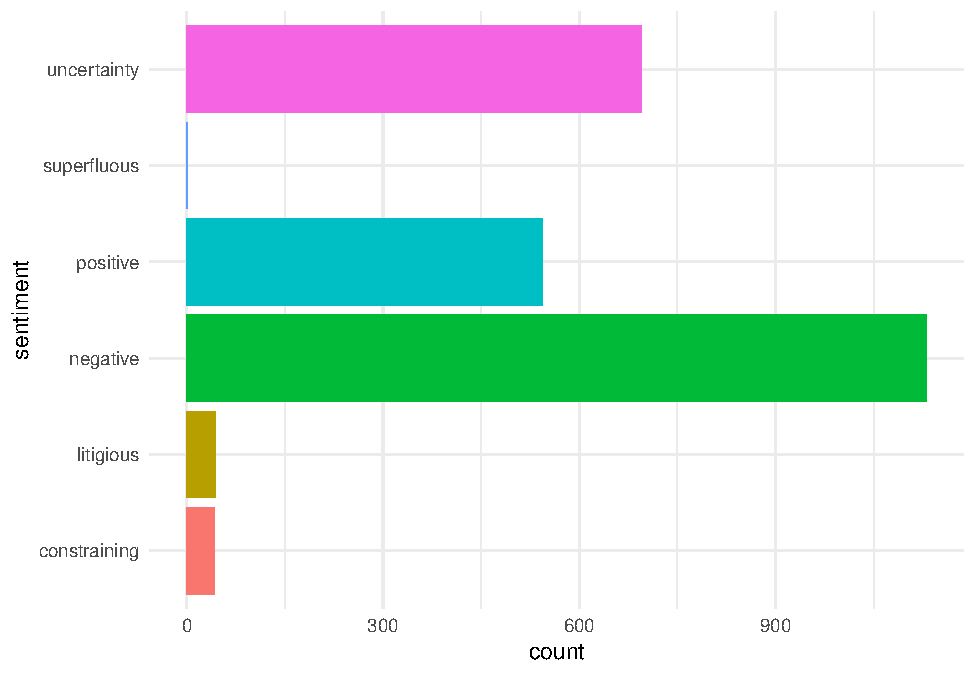
\includegraphics{Final_files/figure-latex/unnamed-chunk-21-1.pdf}

Though is it rudamentary at best, it performs rather well without
needing all of the variables (or further cleaning). Our \(R^2\) value is
hovering around 0.84 and this is with a substantial amount of leverage
and highly unorganized residuals and data. Several of the variables
remain in their original data type when others would be better suited to
modeling. It would also be interesting to include other variables in
this model because again, we simply pulled from the previous one to
scrap together a third model. We finish by making predictions based on
this third model, even though the second one performed better in some
respects such as their coefficients, \(R^2\) and F-statistics.

\begin{Shaded}
\begin{Highlighting}[]
\CommentTok{# Make predictions}
\NormalTok{df <-}\StringTok{ }\NormalTok{test }\OperatorTok\StringTok{ }
\StringTok{  }\NormalTok{dplyr}\OperatorTok{::}\KeywordTok{select}\NormalTok{(}
\NormalTok{            LandSlope,}
\NormalTok{             OverallQual, }
\NormalTok{             KitchenQual, }
\NormalTok{             KitchenAbvGr, }
\NormalTok{             GarageCars,}
\NormalTok{             GarageFinish, }
\NormalTok{             Fireplaces, }
\NormalTok{             YearBuilt, }
\NormalTok{             TotalBsmtSF,  }
\NormalTok{             TotRmsAbvGrd, }
\NormalTok{             SaleType, }
\NormalTok{             GrLivArea, }
\NormalTok{             OverallCond, }
\NormalTok{             LotFrontage,  }
\NormalTok{             Neighborhood)}
\CommentTok{# impute missing values }
\NormalTok{df}\OperatorTok{$}\NormalTok{LotFrontage[}\KeywordTok{is.na}\NormalTok{(df}\OperatorTok{$}\NormalTok{LotFrontage)] <-}\StringTok{ }\KeywordTok{median}\NormalTok{(df}\OperatorTok{$}\NormalTok{LotFrontage, }\DataTypeTok{na.rm =}\NormalTok{ T)}
\NormalTok{df}\OperatorTok{$}\NormalTok{GarageCars[}\KeywordTok{is.na}\NormalTok{(df}\OperatorTok{$}\NormalTok{GarageCars)] <-}\StringTok{ }\KeywordTok{median}\NormalTok{(df}\OperatorTok{$}\NormalTok{GarageCars, }\DataTypeTok{na.rm =}\NormalTok{ T)}
\NormalTok{df}\OperatorTok{$}\NormalTok{TotalBsmtSF[}\KeywordTok{is.na}\NormalTok{(df}\OperatorTok{$}\NormalTok{TotalBsmtSF)] <-}\StringTok{ }\KeywordTok{median}\NormalTok{(df}\OperatorTok{$}\NormalTok{TotalBsmtSF, }\DataTypeTok{na.rm =}\NormalTok{ T)}
\NormalTok{df[df}\OperatorTok{==}\StringTok{'NA'}\NormalTok{] <-}\StringTok{ }\OtherTok{NA}
\NormalTok{df}\OperatorTok{$}\NormalTok{SaleType[}\KeywordTok{is.na}\NormalTok{(df}\OperatorTok{$}\NormalTok{SaleType)] <-}\StringTok{ "WD"}
\NormalTok{df}\OperatorTok{$}\NormalTok{KitchenQual[}\KeywordTok{is.na}\NormalTok{(df}\OperatorTok{$}\NormalTok{KitchenQual)] <-}\StringTok{ "TA"}
\NormalTok{df}\OperatorTok{$}\NormalTok{GarageFinish[}\KeywordTok{is.na}\NormalTok{(df}\OperatorTok{$}\NormalTok{GarageFinish)] <-}\StringTok{ "Unf"}
\NormalTok{predictions <-}\StringTok{ }\KeywordTok{data.frame}\NormalTok{(test}\OperatorTok{$}\NormalTok{Id, }\KeywordTok{predict}\NormalTok{(mod3, df))}
\KeywordTok{colnames}\NormalTok{(predictions) <-}\StringTok{ }\KeywordTok{c}\NormalTok{(}\StringTok{"Id"}\NormalTok{,}\StringTok{"SalePrice"}\NormalTok{)}
\end{Highlighting}
\end{Shaded}

\begin{Shaded}
\begin{Highlighting}[]
\CommentTok{# Export to csv for kaggle submission }
\KeywordTok{write.csv}\NormalTok{(predictions, }\StringTok{"C:/data/predictions.csv"}\NormalTok{)}
\end{Highlighting}
\end{Shaded}

My Kaggle username is ``zacharypalmore'' and my score is 0.17215. This
could have been greatly improved if I had imputed with realistic values
removed missing values prior to each model, considered other variables
beyond these initial thoughts, and much more. Honestly, I am surprised
it turned out as well as it did given the circumstances.

\end{document}
